\documentclass[10pt]{article}
\usepackage{caption}
\usepackage{multirow}
\usepackage{amsfonts}
\usepackage{amsmath}
\usepackage{amssymb}

\usepackage{tikz}
\usepackage{tkz-euclide}
\usetikzlibrary{shapes, backgrounds, calc}
\usetkzobj{all}

\usepackage{hyperref}
\hypersetup{
	colorlinks = true
}

\begin{document}
	\tableofcontents
	\pagebreak

	\section{Review of Propositional Logic}
	\begin{description}
		\item[Task:] Recall enough propositional logic to see how it matches up with set theory.
		\item[Definition:] A \underline{proposition} is any declarative sentence that is either true or false.
	\end{description}
	
	\subsection{Connectives}
	\centerline {
		\begin{tabular}{cccc}
			\multicolumn{3}{c}{\underline{Connectives}} & \multicolumn{1}{c}{\underline{Notation in Maths}} \\
			and & $\land$ \\
			or & $\lor$ & "Inclusive or"\\
			not & $\lnot$ & Sometimes denoted $\sim$\\
			implies & $\to$ & if/then; called implication & $\Rightarrow$\\
			if and only if & $\leftrightarrow$ & Called equivalence & $\Leftrightarrow$\\
		\end{tabular}
	}
	
	\subsubsection{Truth Table of the Connectives}
	Let P, Q be propositions:\\

	\centerline{	
		\begin{tabular}{|c|c|c|}
			\cline{1-3}
			P & Q & P$\land$Q \\ \cline{1-3}
			F & F & F \\ \cline{1-3}
			F & T & F \\ \cline{1-3}
			T & F & F \\ \cline{1-3}
			T & T & T \\ \cline{1-3}
		\end{tabular}
		\quad
		\begin{tabular}{|c|c|c|}
			\cline{1-3}
			P & Q & P$\lor$Q \\ \cline{1-3}
			F & F & F \\ \cline{1-3}
			F & T & T \\ \cline{1-3}
			T & F & T \\ \cline{1-3}
			T & T & T \\ \cline{1-3}
		\end{tabular}
		\quad
		\begin{tabular}{|c|c|}
			\cline{1-2}
			P & $\lnot$P \\ \cline{1-2}
			F & T \\ \cline{1-2}
			T & F \\ \cline{1-2}
		\end{tabular}
		\quad
		\begin{tabular}{|c|c|c|}
			\cline{1-3}
			P & Q & P$\to$Q \\ \cline{1-3}
			F & F & T \\ \cline{1-3}
			F & T & T \\ \cline{1-3}
			T & F & F \\ \cline{1-3}
			T & T & T \\ \cline{1-3}
		\end{tabular}
		\quad
		\begin{tabular}{|c|c|c|}
			\cline{1-3}
			P & Q & P$\leftrightarrow$Q \\ \cline{1-3}
			F & F & T \\ \cline{1-3}
			F & T & F \\ \cline{1-3}
			T & F & F \\ \cline{1-3}
			T & T & T \\ \cline{1-3}
		\end{tabular}
	}
	
	\subsubsection*{Priority of the Connectives}
	\textbf{Highest to Lowest:} $\lnot, \land, \lor, \rightarrow, \leftrightarrow$
	
	\subsection{Important Tautologies}
	\begin{tabular}{rcll}
		$(P \rightarrow Q)$ & $\leftrightarrow$ & $(\lnot P \lor Q)$ \\
		$(P \leftrightarrow Q)$ & $\leftrightarrow$ & $[(P \rightarrow Q) \land (Q \rightarrow P)]$ \\
		$\lnot(P \land Q)$ & $\leftrightarrow$ & $(\lnot P \lor \lnot Q)$ & \multirow{2}{4cm}{\LARGE\} \normalsize De Morgan Laws} \\
		$\lnot(P \lor Q)$ & $\leftrightarrow$ & $(\lnot P \land \lnot Q)$ \\
	\end{tabular}
	~\\~\\~\\
	As a result, $\lnot$ and $\lor$ together can be used to represent all of $\lnot, \land, \lor, \rightarrow, \leftrightarrow$.
	
	\begin{description}
		\item[Less obvious:] One connective called the sheffer stroke P$\mid$Q (which stands for "not both P and Q" or "P nand Q") can be used to represent all of $\lnot$, $\land$, $\lor$, $\rightarrow$, $\leftrightarrow$ since $\lnot$P $\leftrightarrow$ P$\mid$P and P $\lor$ Q $\leftrightarrow$ (P$\mid$P) $\mid$ (Q$\mid$Q).
		\item[Recall] if P$\rightarrow$Q is a given implication, Q$\rightarrow$P is called the \underline{converse} or P$\rightarrow$Q. $\lnot$Q $\rightarrow$ $\lnot$P.
	\end{description}
	
	\subsection{Indirect Arguments/Proofs by Contradiction/Reductio as absurdum}
	Based on the tautology (P$\rightarrow$Q) $\leftrightarrow$ ($\lnot$Q $\rightarrow$ $\lnot$P)
	
	\begin{description}
		\item[Example:] Famous argument that $\sqrt{2}$ is irrational.
		\item[Proof:]
		\item \textbf{Suppose} $\sqrt{2}$ is rational, then it can be expressed is fraction form $\frac{a}{b}$. Let us \textbf{assume} that our fraction is in the lowest term, \textbf{i.e.} their only common divisor is 1.
		\item Then, \[\sqrt{2}=\frac{a}{b}\]
		\item Squaring both sides, we have \[2=\frac{a^2}{b^2}\]
		\item Multiplying both sides by $B^2$ yields \[2b^2=a^2\]
		\item Since $a^2b^2$, we can conclude that $a^2$ is even because whatever the value of $b^2$ has to be multiplied by 2. If $a^2$ is even, then $a$ is also even. Since $a$ is even, no matter what the value of $a$ is, we can always find an integer that if we divide $a$ by 2, it is equal to that integer. If we let that integer be $k$, then $\frac{a}{b}=k$ which means that $a=2k$.
		\item Substituting the value of $2k$ to $a$, we have $2b^2=(2k)^2$ which means that $2b^2=4k^2$. dividing both sides by 2 we have $b^2=2k^2$. That means that the value $b^2$ is even, since whatever the value of $k$ you have to multiply it by 2. Again, is $b^2$ is even, then $b$ is even.
		\item This implies that both $a$ and $b$ are even, which means that both the numerator and the denominator of our fraction are divisible by 2. This contradicts our \textbf{assumption} that $\frac{a}{b}$ has no common divisor except 1. Since we found a contradiction, our assumption is, therefore, false. Hence the theorem is true.
		\item \textbf{qed}
	\end{description}
	
	\section{Predicate logic and Quantifiers}
	\begin{description}
		\item[Task:] Understand enough predicate logic to make sense of quantified statements.
		\item In predicate logic, propositions depend on variable x, y, z, so their truth value may change depending on which values these variables assume: $P(x), Q(x, y), R(x, y, z)$
	\end{description}
	
	\subsection{Introduce quantifiers}
	\subsubsection{$\exists$ existential quantifier}
	\begin{description}
		\item[Syntax:] $\exists xP(x)$
		\item[Definition:] $\exists xP(x)$ is true if $P(x)$ is true or some value of $x$; it is false otherwise.
	\end{description}
	
	\subsubsection{$\forall$ universal quantifier}
	\begin{description}
		\item[Syntax:] $\forall xP(x)$
		\item[Definition:] $\forall xP(x)$ is true if $P(x)$ is true for all allowable values of $x$. It is false otherwise.
	\end{description}
	
	\subsubsection{$\exists!$ for one and only one}
	\begin{description}
		\item[Syntax:] $\exists! xP(x)$
		\item[Definition:] $\exists! xP(x)$ is true if $P(x)$ is true for exactly one value of $x$ and false for all often values of $x$; otherwise, $\exists! xP(x)$ is false.
	\end{description}
	
	\subsection{Alternation of Quantifiers}
	\begin{tabular}{lr}
		$\forall x\exists y\forall z$ & $P(x, y, z)$ \\
	\end{tabular}
	~\\
	\textbf{NB:} The order \underline{cannot} be exchanged as it might modify the truth values of the statement (think of examples with two quantifiers).
	
	\subsection{Negation of Quantifiers}
	\begin{tabular}{rcl}
		$\lnot(\exists xP(x))$ & $\leftrightarrow$ & $\forall x\lnot P(x)$ \\
		$\lnot(\forall xP(x))$ & $\leftrightarrow$ & $\exists x\lnot P(x)$ \\
	\end{tabular}
	
	\section{Set Theory}
	\begin{description}
		\item[Task:] Understand enough set theory to make sense of other mathematical objects in abstract algebra, graph theory, etc. Set theory started around 1870's $\rightarrow$ late development in mathematics but now taught early in one's maths education due to Bourbaki school.
		\item[Definition:] A set is a collection of objects. $x\in A$ means the element $X$ is in the set $A$ (\textbf{i.e.} belongs to $A$).
		\item[Examples:] 
		\begin{enumerate}
			\item[]
			\item All students in a class.
			\item $\mathbb{N}$ the set of natural numbers starting at 0.
			\begin{enumerate}
				\item [$\mathbb{N}$] is defined via the following two axioms:
				\item 0 $\in \mathbb{N}$
				\item if $x \in \mathbb{N}$ then $x+1 \in \mathbb{N}$ ($x \in \mathbb{N} \rightarrow X+A \in \mathbb{N}$)
			\end{enumerate}
			\item $\mathbb{R}$ set of real numbers also introduced axiomatically
			\begin{enumerate}
				\item[$\mathbb{R}$] the set of real numbers.
				\item Additive closure: $\forall x, y \exists z (x+y=z)$
				\item Multiplicative closure: $\forall x, y, \exists z (x \times y=z)$
				\item Additive associativity: $x+(y+z)=(x+y)+z$
				\item Multiplicative associativity: $x \times (y \times z) = (x \times y) \times z$
				\item Additive commutativity: $x+y=y+x$
				\item Multiplicative commutativity: $x \times y = y \times x$
				\item Distributivity: $x \times (y+z) = (x \times y) + (x \times z)$ and $(y+z) \times x = (y \times x) + (z \times x)$
				\item Additive identity: There is a number, denoted 0, such that or all $x, x+0=x$
				\item Multiplicative identity: There is a number, denoted 1, such that for all $x, x \times 1 = 1 \times x = x$
				\item Additive inverses: For every $x$ there is a number, denoted $-x$, such that $x+(-x)=0$
				\item Multiplicative inverses: For every nonzero $x$ there is a number, denoted $x$, such that $x \times x^{-1} = x^{-1} \times x = 1$
				\item $0 \neq 1$
				\item Irreflexivity of $<: \sim (x<x)$
				\item Transitivity of <: If $x<y$ and $y<z$, then $x<z$
				\item Trichotomy: Either $x<y, y<x,$ or $x=y$
				\item If $x<y$, then $x+y<y+z$
				\item If $x<y$ and $0<z$, then $x \times z < y \times z$ and $z \times x < z \times y$
				\item Completeness: If a nonempty set of real numbers has an upper bound, then it has a \textit{least} upper bound.
			\end{enumerate}
			\item $\emptyset$ is the empty set (The set with no elements).
		\end{enumerate}
		\item[Definition:] Let A, B be sets. A=b if and only if all elements of A are elements of B and all elements of B are elements of A,\\i.e. $A=b \leftrightarrow [\forall x (x \in A \rightarrow x \in B)] \cap [\forall y (y \in B \rightarrow y \in A)]$
	\end{description}
		
	\subsection{Two Ways to Describe Sets}
	\begin{enumerate}
		\item The enumeration/roster method: list all elements of the set.\\ \textbf{NB:} order is \underline{irrelevant}.\\ $A=\{0, 1, 2, 3, 4, 5\}=\{5, 0, 2, 3, 1, 4\}$
		\item The formulaic/set builder method: give a formula that generates all elements of the set.\\ $A=\{x \in \mathbb{N} \mid 0 \leq x \land x \leq 5\} = \{0, 1, 2, 3, 4, 5\} = \{x \in \mathbb{N} : 0 \leq x \land x \leq 5 \}$
	\end{enumerate}
	Using $\mathbb{N}$ and the set-builder method, we can define:
		
	$\mathbb{Z} = \{m-n \mid \forall m, n \in \mathbb{N} \}$
		
	\hspace{5mm} $n=0$ in any natural numbers $\Rightarrow$ we generate all of $\mathbb{N}$
		
	\hspace{5mm} $m=0$ in any natural number $\Rightarrow$ we generator all negative integers
		
	$\mathbb{Q} = \{\frac{p}{q} \mid p, q \in \mathbb{Z} \land q \neq 0 \}$
	\begin{description}
		\item[Definition:] A set $A$ is called finite if it has a finite number of elements; otherwise it is called infinite.
	\end{description}
		
	\section{Set Operations}
	\begin{description}
		\item[Task:] Understand how to represent sets by Venn diagrams. Understand set union, intersection, complement and difference.
		\item[Definition:] Let $A, B$ be sets. $A$ is a \underline{subset} of $B$. If all elements of $A$ are elements of $B$, \textbf{i.e.} $\forall x(x \in A \rightarrow x \in B)$. We denote that $A$ is a subset of $B$ by $A \subseteq B$
		\item[Example:] $\mathbb{N} \subseteq \mathbb{Z}$
		\item[Definition:] Let $A, B$ be sets. $A$ is a \underline{proper} subset of $B$ if $A \subseteq B \land A \neq B$, \textbf{i.e.} $A \subseteq B \land \exists x \in B s.t. x \notin A$. \\ A proper subset is always a subset, but a subset is not always a proper subset.
		\item[Notation:] $A \subset B$
		\item[Example:] $\mathbb{N} \subset \mathbb{Z}$ since $\exists -1 \in \mathbb{N}$ \\ \textbf{NB:} $\forall A$ a set $\emptyset \subseteq A$
		\item[Recall:] $B \subseteq C$ means $\forall x(x \in B \rightarrow x \in C)$, but $\emptyset$ has no elements so in $\emptyset \subseteq A$ the quantifier $\forall$ operates on a domain with no elements. Clearly, we need to give meaning to $\exists$ and $\forall$ on empty sets.
	\end{description}
	
	\begin{tabular}{cc}
		\underline{Boolean Convention} \\
		$\forall$ is true on the empty set & \multirow{2}{6cm}{\LARGE\} \normalsize Consistent with common sense} \\
		$\exists$ is false on the empty set
	\end{tabular}
	
	\begin{description}
		\item[Definition:] Let $A, B$ be two sets. The \underline{union} $A \cup B = \{x \mid x \in A \lor x \in B \}$
		\item[Definition:] Let $A, B$ be two sets. The \underline{intersection} $A \cap B = \{x \mid x \in A \land x \in B \}$
		\item[Definition:] Let $A, B$ be sets. $A$ and $B$ are called \underline{disjoint} is $A \cap B = \emptyset$
		\item[Definition] Let $A, B$ be two sets. $A-B = A \backslash B = \{a \mid x \in A \land x \notin B \}$
		\item[Examples:]
		\begin{tabular}{ll}
			$A = \{1, 2, 5\}$ & $B = \{1, 3, 6\}$ \\
			$A \cup B = \{1, 2, 3, 5, 6\}$ & $A \cap B = \{1\}$ \\
			$A \backslash B = \{2, 5\}$ & $B \backslash A = \{3, 6\}$ \\
		\end{tabular}
		\item[Definition:] Let $A, U$ be sets s.t. $A \subseteq U$. The \underline{complement} of $A$ in $U$ = $U \backslash A = A^C = \{x \mid x \in U \land x \notin A \}$
		\item[Remark:] The notation $A^C$ is unambiguous only if the universe U is clearly defined or understood.
	\end{description}
	
	\subsection{Venn Diagrams}
	Schematic representation of set operations. \\

	\begin{figure}[h]
		\centering
		\def \setu{(0, 0)rectangle(4.5, 3)}
		\def \seta{(1.5, 1.5)circle(1)}
		\def \setb{(3, 1.5)circle(1)}
		\begin{tikzpicture}
			
			\begin{scope}
				\draw \seta node{$A$};
				\draw \setb node{$B$};
				\draw \setu;
			\end{scope}
			
			\begin{scope}[shift={(5cm, 0cm)}, even odd rule]
				\draw \seta node{$A$};
				\draw \setb node{$B$};
				\draw \setu (2.25, -0.5) node{$A^C$};
				\clip \seta \setu;
				\filldraw[red, fill opacity=0.5] \setu;
			\end{scope}
			
			\begin{scope}[shift={(0cm, -4cm)}]
				\draw \seta node{$A$};
				\draw \setb node{$B$};
				\draw \setu (2.25, -0.5) node{$A \cap B$};
				\clip \seta;
				\filldraw[red, fill opacity=0.5] \setb;
			\end{scope}
			
			\begin{scope}[shift={(5cm, -4cm)}]
				\draw \seta node{$A$};
				\draw \setb node{$B$};
				\draw \setu (2.25, -0.5) node{$A \cup B$};
				\filldraw[red, fill opacity=0.5] \seta \setb;
			\end{scope}

			\begin{scope}[shift={(0cm, -8cm)}, even odd rule]
				\draw \seta node{$A$};
				\draw \setb node{$B$};
				\draw \setu (2.25, -0.5) node{$A \backslash B$};
				\clip \seta \setb;
				\filldraw[red, fill opacity=0.5] \seta;
			\end{scope}
			
			\begin{scope}[shift={(5cm, -8cm)}, even odd rule]
				\draw \seta node{$A$};
				\draw \setb node{$B$};
				\draw \setu (2.25, -0.5) node{$B \backslash A$};
				\clip \seta \setb;
				\filldraw[red, fill opacity=0.5] \setb;
			\end{scope}
		\end{tikzpicture}
	\end{figure}

	\newpage
	\subsection{Properties of Set Operations}
	\begin{table}[h!]
		\centering
		\caption*{Correspondence between Logic and Set Theory}
		\begin{tabular}{|c|c|}
			\cline{1-2}
			Logical Connective & Set operation \\ \cline{1-2}
			$\land$ & intersection $\cap$ \\ \cline{1-2}
			$\lor$ & union $\cup$ \\ \cline{1-2}
			$\lnot$ & complement $(~)^C$ \\ \cline{1-2}
		\end{tabular}
	\end{table}
	~\\
	As a result, various properties of set operations become obvious:
	\begin{itemize}
		\item Commutativity
		\begin{itemize}
			\item $A \cap B = B \cap A$
			\item $A \cup B = B \cup A$
		\end{itemize}
		\item Associativity
		\begin{itemize}
			\item $(A \cup B) \cup C = A \cup (B \cup C)$
			\item $(A \cap B) \cap C = A \cap (B \cap C)$
		\end{itemize}
		\item Distributivity
		\begin{itemize}
			\item $A \cap (B \cup C) = (A \cap B) \cup (A \cap C)$
			\item $A \cup (B \cap C) = (A \cup B) \cap (A \cup B)$
		\end{itemize}
		\item De Morgan Laws in Set Theory
		\begin{itemize}
			\item $(A \cap B)^C = A^C \cup B^C$
			\item $(A \cup B)^C = A^C \cap B^C$
		\end{itemize}
		\item Involutivity of the Complement
		\begin{itemize}
			\item $(A^C)^C = A$
		\end{itemize}
		\item[\textbf{NB:}] An involution is a map such that applying it twice gives the identity. Familiar examples: reflecting across the x-axis, the y-axis, or the origin in the plane.
		\item Transitivity of Inclusion
		\begin{itemize}
			\item $A \subseteq B \land B \subseteq C \rightarrow A \subseteq C$
		\end{itemize}
		\item Criterion for proving equality of sets
		\begin{itemize}
			\item $A=B \leftrightarrow A \subseteq C \land B \subseteq A$
		\end{itemize}
		\item Criterion for proving non-equality of sets
		\begin{itemize}
			\item $A \neq B \leftrightarrow (A \backslash B) \cup (B \backslash A) \neq 0$
		\end{itemize}
	\end{itemize}
	
	\subsection{Example Proof in Set Theory}
	\begin{description}
		\item[Proposition:] $\forall A, B$ sets. $(A \cap B) \cup (A \backslash B) = A$
		\item[Proof:] Use the criterion for proving equality of sets from above, \textbf{i.e.} inclusion in both directions.
		\item \underline{Show $(A \cap B) \cup (A \backslash B) \subseteq A$:} $\forall x \in (A \cap B) \cup (A \backslash B), x \in (A \cap B)$ or $x \in A \backslash B$. If $x \in (A \cap B)$ then clearly $x \in A$ as $A \cap B \subseteq A$ by definition. If $x \in A \backslash B$, then by definition $x \in A$ and $x \notin B$ so definitely $x \in A$. In both cases, $x \in A$ as needed.
		\item \underline{Show $A \subseteq (A \cap B) \cup (A \backslash B)$:} $\forall x \in A$, we have two possibilities, namely $x \in B$ or $x \notin B$. If $x \in B$, then $x \in A$ and $x \in B$, so $x \in A \cap B$. If $x \notin B$, then $x \in A$ and $x \notin B$, so $x \notin A \backslash B$. In both cases, $x \in (A \cap B)$ or $x \in (A \backslash B)$ so $x \in (A \cap B) \cup (A \backslash B)$ as needed.
		\item \textbf{qed}
	\end{description}
	
	\section{The Power Set}
	\begin{description}
		\item[Task:] Understand what the power set of a set $A$ is.
		\item[Definition:] Let $A$ be a set. The power set of $A$ denoted $P(A)$ is the collection of all the subsets of $A$.
		\item[Recall:] $\emptyset \subseteq A$. It is also clear from the definition of a subset that $A \subseteq A$.
		\item[Examples:]
		\begin{enumerate}
			\item[]
			\item $A=\{0, 1\}$ \\
			$P(A) = \{\emptyset, \{0\}, \{1\}, \{0, 1\} \}$
			\item $A=\{a, b, c\}$ \\
			$P(A) = \{\emptyset, \{a\}, \{b\}, \{c\}, \{a, b\}, \{a, c\}, \{b, c\}, \{a, b, c\} \}$
			\item $A = \emptyset$ \\
			$P(A) = \{\emptyset\}$ \\
			$P(P(A)) = \{\emptyset, \{\emptyset\} \}$
			\item [\textbf{NB:}] $\emptyset$ and $\{\emptyset\}$ are different objects. $\emptyset$ has no elements, whereas $\{\emptyset\}$ has one element.
		\end{enumerate}
		\item[Remark:] $P(A)$ and $A$ are viewed as living in separate worlds to avoid phenomena like Russell' paradox.
		\item[Q:] If $A$ has $n$ elements, how many elements does $P(A)$ have?
		\item[A:] $2^n$
		\item[Theorem:] Let $A$ be a set with $n$ elements, then $P(A)$ contains $2^n$ elements.
		\item[Proof:] Based on the on/off switch idea.
		\item $\forall x \in A$, we have two choices: either we include $x$ in the subset or we don't (on vs off switch). $A$ has $n$ elements $\Rightarrow$ we have $2^n$ subsets of $A$.
		\item \textbf{qed}
		\item [Alternate Proof:] Using mathematical induction. \\
		\textbf{NB:} It is an axiom of set theory (in the ZFC standard system) that every set has a power set, which implies no set consisting of all possible sets could limit, else what would its power set be?
	\end{description}
	
	\section{Cartesian Products}
	\begin{description}
		\item[Task:] Understand sets like $\mathbb{R}^1$ in a more theoretical way.
		\item[Recall from Calculus:]
		\item $\mathbb{R} = \mathbb{R}^1 \ni x$
		\item $\mathbb{R} \times \mathbb{R} = \mathbb{R}^2 \ni (x_1, x_1)$ \\ \vdots
		\item $\underbrace{\mathbb{R} \times \mathbb{R}}_{\text{n times}} = \mathbb{R}^2 \ni (x_1, x_2, ..., x_n)$
		\item These are examples of Cartesian products.
		\item[Definition:] Let $A, B$ be sets. The Cartesian product denoted by $A ]times B$ consists of all ordered pairs $(x, y) st x \in A \land y \in B$, \textbf{i.e.} $A \times B = \{(x, y) \mid x \in A \land y \in B \}$
		\item[Further Examples:]
		\begin{enumerate}
			\item[]
			\item $A = \{1, 3, 7\}$ \\
			$B = \{1, 5\}$ \\
			$A \times B = \{(1, 1), (1, 5), (3, 1), (3, 5), (7, 1), (7, 5)\}$ \\
			\textbf{NB:} The order in which elements in a pair matters: $(7, 1)$ is different from $(1, 7)$. This is why we call $(x, y)$ an \underline{ordered} pair.
			\item $A = \{(x, y) \in \mathbb{R}^ \mid x^2 + y^2 = 1 \} \leftarrow$ circle of radius 1 \\
			$B = \{z \in \mathbb{R} \mid -2 \leq z \leq 2 \} = \{-2, 2\} \leftarrow$ closed interval \\
			$A \times B \leftarrow$ cylinder of radius 1 and height 4
		\end{enumerate}
	\end{description}
	
	\subsection{Cardinality (number of elements) in a Cartesian product}
	If $A$ has $n$ elements and $B$ has $p$ elements, $A \times B$ has $np$ elements.
	\pagebreak
	\begin{description}
		\item[Example:]
		\begin{enumerate}
			\item[]
			\item $ \#(A) = 3 \hspace{10mm} A = \{1, 3, 7\}$ \\
			$\#(B) = 2 \hspace{10mm} B = \{1, 5\}$ \\
			$\#(A) \times B) = 3 \times 2 = 6$
			\item Both $A$ and $B$ are infinite sets, so $A \times B$ is infinite as well.
		\end{enumerate}
		\item[Remark:] We can define Cartesian products of any length, \textbf{e.g.} $A \times A \times B \times A$, $B \times A \times B \times A \times B$, etc. If all sets are finite, the number of elements is the product of the numbers of elements of each factor. If $\#(A) = 3$ and $\#(B) = 2$ as above, $\#(A \times B ]times A) = 3 \times 3 \times 3 = 18$ and $\#(B \times A \times B) = 2 \times 3 \times 2 = 12$.
	\end{description}
	
	\section{Relations}
	\begin{description}
		\item[Task:] Define subsets of Cartesian products with certain properties. Understand the predicates $"="$ (equality) and other predicates in predicate logic in a more abstract light.
		\item Start with $x=y$. The elements $x$ is some notation $R$ to $y$ (equality in this case). We can also denote it as $xRy$ or $(x, y) \in E)$
		\item Let $x, y$ in $\mathbb{R}$, then $E = \{(x, x) \mid x \in \mathbb{R} \} \subset \mathbb{R} \times \mathbb{R}$.
		\item The "diagonal" in $\mathbb{R} \times \mathbb{R}$ gives exactly the elements equal to each other.
		\item More generally:
		\item[Definition:] Let $A, B$ be sets. A subset of the Cartesian product $A \times B$ is called a relations between $A$ and $B$. A subset of the Cartesian product $A \times A$ is called a relations on $A$.
		\item[Remark:] Note how general this definition is. To make it useful for understanding predicates, we will need to introduce key properties relations can satisfy.
		\item[Example:] $A = \{1, 3, 7\} \hspace{10mm} B = \{1, 2, 5\}$
		\item We can define a relation $S$ on $A \times B$ by $S = \{(1, 1), (1, 5), (3, 2)\}$. This means $1S1$, $1S5$ and $3S2$ and no other ordered pairs in $A \times B$ satisfy $S$.
		\item[Remark:] The relations we defined involve 2 elements, so they are often called \underline{binary relations} in the literature.
	\end{description}
	
	\section{Equivalence Relations}
	\begin{description}
		\item[Task:] Define the most useful kind of relation.
		\item[Definition:] A relation $R$ on a set $A$ is called
		\begin{enumerate}
			\item \underline{reflexive} iff (if and only if) $\forall x \in A, xRx$
			\item \underline{symmetric} iff $\forall x, y \in A, xRy \rightarrow yRx$
			\item \underline{transitive} iff $\forall x, y, z \in A, xRy \land yRz \rightarrow xRz$
		\end{enumerate}
		\item An equivalence relation on $A$ is a relation that is reflexive, symmetric and transitive.
		\item[Notation:] Instead of $xRy$, an equivalence relation is often denoted by $x \equiv y$ or $x \sim y$.
		\item[Examples:]
		\begin{enumerate}
			\item[]
			\item "=" equality is an equivalence relation.
			\begin{enumerate}
				\item $x=x$ reflexive
				\item $x=y \Rightarrow y=x$ symmetric
				\item $x=y \land y=z \Rightarrow x=z$ transitive 
			\end{enumerate}
			\item $A = \mathbb{N} \\
			x \equiv y$ mod $3$ is an equivalence relation. $x \equiv y$ mod 3 means $x-y = 3m$ for some $m \in \mathbb{Z}$, \textbf{i.e.} $x$ and $y$ have the same remainder when divided by 3. The set of all possible remainders is $\{0, 1, 2\}$ \\
			\textbf{NB:} In correct logic notation, $x \equiv y$ mod 23 if $\exists m \in \mathbb{Z} s.t. x-y=3m$
			\begin{enumerate}
				\item $x \equiv x$ mod 3 since $x-x=0=3 \times 0 \rightarrow$ reflexive
				\item $x \equiv y$ mod 3 $\Rightarrow y \equiv x$ mod 3 because $x \equiv y$ mod 3 means $x-y=3m$ for some $m \in \mathbb{Z} \Rightarrow y-x=-3m=3 \times (-m) \Rightarrow y \equiv x$ mod 3 $\rightarrow$ symmetric
				\item Assume $x \equiv y$ mod 3 and $y \equiv z$ mod 3 \\
				$x \equiv y$ mod 3 $\Rightarrow \exists m \in \mathbb{Z}$ s.t. $x-y=3m \Rightarrow y=x-3m$ \\
				$y \equiv z$ mod 3 $\Rightarrow \exists p \in \mathbb{Z}$ s.t. $y-z=3p \Rightarrow y=z+3p$ \\
				Therefore, $x-3m=z+3p \Leftrightarrow x-z=3p+3m = 3(p+m)$ \\
				Since $p, m \in \mathbb{Z}, p+m \in \mathbb{Z} \Rightarrow x \equiv z$ mod 3 $\rightarrow$ transitive.
			\end{enumerate}
			\item Let $f:A \rightarrow A$ be any function on a non empty set A. We define the relation $R = \{(x, y) \mid f(x)=f(y) \}$
			\begin{enumerate}
				\item $\forall x \in A, f(x)=f(x) \Rightarrow (x, x) \in R \rightarrow reflexive$
				\item If $(x, y) \in R$, then $f(x)=f(y) \Rightarrow f(y)=f(x)$, \textbf{i.e.} $(y, x) \in R \rightarrow$ symmetric
				\item If $(x, y) \in R$ and $(y, z) \in R$, then $f(x)=f(y)$ and $f(y)=f(z)$, which by the transitivity of equality implies $f(x)=f(z)$, \textbf{i.e.} $(x, z) \in R$ as needed, so $R$ is transitive as well.\\
				$f(x)$ can be $e^x, sin\:x, (x)$, etc.
			\end{enumerate}
			\pagebreak
			\item Let $\lambda$ be the set of all triangles in the plane. $ABC \sim A'B'C'$ if $ABC$ and $A'B'C'$ are similar triangles, \textbf{i.e.} have equal angles.
			
			\begin{figure}[t!]
				\centering
				\begin{tikzpicture}
					\coordinate (A) at (0, 0);
					\coordinate (B) at (1, 1);
					\coordinate (C) at (2, 0);
					\draw (A)--(B)--(C)--cycle;

					\tkzLabelAngle[pos = 0.4](B,A,C){A}
					\tkzLabelAngle[pos = 0.4](A,B,C){B}
					\tkzLabelAngle[pos = 0.4](A,C,B){C}
					
					\coordinate (A') at (3, 0);
					\coordinate (B') at (5, 2);
					\coordinate (C') at (7, 0);
					
					\draw (A')--(B')--(C')--cycle;
					
					\tkzLabelAngle[pos = 0.5](B',A',C'){A'}
					\tkzLabelAngle[pos = 0.5](A',B',C'){B'}
					\tkzLabelAngle[pos = 0.5](A',C',B'){C'}
				\end{tikzpicture}
			\end{figure}
			
			\begin{enumerate}
				\item $\forall ABC \in \lambda, ABC \sim ABC$ so $\sim$ is reflexive
				\item $ABC \sim A'B'C' \Rightarrow A'B'C' \sim ABC$ so $\sim$ is symmetric
				\item $ABC \sim A'B'C'$ and $A'B'C' \sim A"B"C" \Rightarrow ABC \sim A"B"C"$, so $\sim$ is transitive
				\item[Clearly] (a), (b), (c) use the fact that equality of angles is an equivalence relation.
			\end{enumerate}
		\end{enumerate}
		\item[Exercise:] For various predicates you've encountered, check whether reflexive, symmetric or transitive. Examples of predicates include $\neq, <, >, \leq, \geq, \subseteq$
	\end{description}
	
	\section{Equivalence Relations and Partitions}
	\begin{description}
		\item[Task:] Understand how equivalence relations divide sets.
		\item[Definition:] Let $A$ be a set. A \underline{partition} of $A$ is a collection of non empty sets, any two of which are disjoint such that their union is $A$, \textbf{i.e.} $\lambda = \{A_\alpha \mid \alpha \in I \}$ s.t. $\forall \alpha , \alpha ' \in I$ satisfy $\alpha \neq \alpha ', A_\alpha \cap A_{\alpha '} \neq \emptyset$ and $\underset{\alpha \in I}{\cup} A_\alpha = A$
		\item Here $I$ is an indexing act (may be infinite). $\underset{\alpha \in I}{A_\alpha}$ is the union of all the $A_\alpha$'s (possibly an infinite union)
		\item[Example] $\{(n, n+1) \mid n \in \mathbb{Z} \}$ is a partition of $\mathbb{R}$
		\begin{figure}[h]
			\centering
			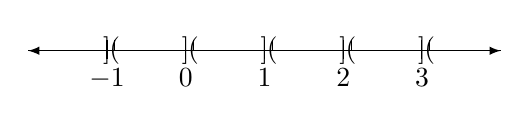
\begin{tikzpicture}
				\draw[latex-] (-2, 0) -- (4, 0);
				\draw[-latex] (-2, 0) -- (4, 0);
				
				% lines on numberline
				\foreach \x in {-1, 0, 1, 2, 3}
				\draw[shift={(\x, 0)}, color=black] (0pt, 3pt) -- (0pt, -3pt);
				
				%numbers on numberline
				\foreach \x in {-1, 0, 1, 2, 3}
				\draw[shift={(\x, 0)}, color=black] (0pt, 0pt) -- (0pt, -3pt) node[below] {$\x$};
				
				\foreach \x in {-0.9, 0.1, 1.1, 2.1, 3.1}
				\draw[shift={(\x, 0)}, color=black] (0pt, 4pt) -- (0pt, 0pt) node {{}(};
				\foreach \x in {-1, 0, 1, 2, 3}
				\draw[shift={(\x, 0)}, color=black] (0pt, 4pt) -- (0pt, 0pt) node {{}]};
			\end{tikzpicture}
		\end{figure}
		\item $\underset{n \in \mathbb{Z}}{\cup} (n, n+1 ] = \mathbb{R}$
		\item $(n, n+1 ] \cap (m, m+1 ] = \emptyset$ if $n \neq m$
		\item[Definition:] If $R$ is an equivalence relations on a set $A$ and $x \in A$, the equivalence class of $x$ denoted $[x]_R$ is the set $\{y \mid xRy \}.$ The collection of all equivalence classes is called $A$ modulo $R$ and denoted $A/R$.
		\item[Examples:]
		\begin{enumerate}
			\item[]
			\item $A = \mathbb{N} \hspace{10mm} x \equiv y$ mod 3 \\
			We have the equivalence classes $[0]_R, [1]_R$ and $[2]_R$ given by the then possible remainders under division by 3. \\
			${[0]}_R = \{0, 3, 6, 9, ...\}$ \\
			${[1]}_R = \{1, 4, 7, 10, ...\}$ \\
			${[2]}_R = \{2, 5, 8, 11, ...\}$ \\
			Clearly ${[0]}_R \cup {[1]}_R \cup {[2]}_R = \mathbb{N}$ and they are mutually disjoint $\Rightarrow R$ gives a partition of $\mathbb{N}$.
			\item $ABC \sim A'B'C'$ \\
			$[ABC] = \{$The set of all triangles with angles of magnitude $\measuredangle{ABC}, \measuredangle{BAC}, \measuredangle{ACB} \}$ \\
			The union over the set of all $[ABC]$ is the set of all triangles and $[ABC] \cap [A'B'Ç'] = \emptyset$ if $ABC \neq ^* A'B'C'$ since it means these triangles have at least one angle that if difference.
			\item [$^*$] In the original notes, not $\sim$ is used (a tilde with a slash going through it) but I couldn't find this symbol in latex.
			\item $A = \mathbb{C} \hspace{10mm} x \cap y$ if $|x| = |y|$ \hspace{10mm} equivalence relation \\
			$[x] = \{y \in \mathbb{C} \mid |x|=|y| \} = [r]$ for $r \in [0, +\infty) \land (r \geq 0)$ \\
			\begin{figure}[h]
				\centering
				\caption*{circle of radius $|x|$}
				\begin{tikzpicture}
					\draw(3, 0) -- (-3, 0) node[left]{Real};
					\draw(0, -3) -- (0, 3) node[above]{Imaginary};
					\draw{(0, 0)circle(2)};
				\end{tikzpicture}
			\end{figure}
			\\
			$\underset{r \in [0, +\infty)}{\cup} [r] = \mathbb{C}$ \\
			$[r_1] \cap [r_2] \neq \emptyset$ if $r_1 \neq r_2$ since two distinct circles in $\mathbb{C} \simeq \mathbb{R}^2$ with empty intersection.
			\pagebreak
			\begin{figure}[h]
				\centering
				\caption*{circles $r_1 \land r_2$}
				\begin{tikzpicture}
				\draw(-3, 0) -- (3, 0);
				\draw(0, -3) -- (0, 3);
				\draw{(0, 0)circle(2)};
				\draw{(0, 0)circle(1)};
				\end{tikzpicture}
			\end{figure}
		\end{enumerate}
		\item[Theorem:] For any equivalence relation $R$ on a set $A$, its equivalence classes form a partition of $A$, \textbf{i.e.}
		\begin{enumerate}
			\item $\forall x \in A, \exists y \in A$ s.t. $x \in [y]$ (every element of $A$ sits somewhere)
			\item $xRy \Leftrightarrow [x]=[y]$ (all elements related by $R$ belong to the same equivalence class)
			\item $\lnot (xRy) \Leftrightarrow [x] \cap [y] = \emptyset$ (if two elements are not related by $R$, the they belong to disjoint equivalence classes)
		\end{enumerate}
		\item[Proof:]
		\begin{enumerate}
			\item[]
			\item Trivial. Let $y=x$. $x \in [x]$ because $R$ is an equivalence relation. Hence reflexive, so $xRx$ holds.
			\item We will prove $xRy \Leftrightarrow [x] \subseteq [y]$ and $[y] \subseteq [x]$ \\
			$\Rightarrow$ Fix $x \in A, [x] = \{z \in A \mid xRz \} \Rightarrow \forall y \in A$ s.t. $xRy, y \in [x]$. Furthermore, $[y] = \{w \in A \mid yRw \}$ \\
			$\Rightarrow \forall w \in [u], yRw$ but $xRy \Rightarrow xRw$ by transitivity. Therefore, $w \in [x]$. We have shown $[y] \subseteq [x]$. \\
			Since $R$ is an equivalence relation, it is also symmetric. \textbf{i.e.} $xRy \Leftrightarrow yRx$. So by the same argument with $x$ and $y$ swapped $yRx \Rightarrow [x] \subseteq [y]$. Thus $xRy \Rightarrow [x] = [y]$. \\
			$\Rightarrow [x]=[y] \Rightarrow y \in [x]$ but $[x] = \{y \in A \mid xRy \}$
			\item $\Rightarrow$ We will prove the contrapositive. Assume $[x] \cap [y] \neq \emptyset \Rightarrow \exists z \in [x] \cap [y]. z \in [x]$ means $xRy$, whereas $z \in [y]$ means $yRx \Leftrightarrow zRy$ by symmetric of $R$. We thus have $xRz$ and $zRy \Rightarrow xRy$ by transitivity of $R. xRy$ contradicts $\lnot(xRy)$ so indeed $\lnot(xRy) \Rightarrow [x] \cap [y] = \emptyset$ \\
			$\Leftarrow$ Once again we use the contrapositive. \\
			Assume $\lnot(\lnot(xRy)) \Leftrightarrow xRy$. By part (b) $xRy \Rightarrow [x] = [y] \Rightarrow [x] \cap [y] \neq \emptyset$ since $x \in [x]$ and $y \in [y]$, \textbf{i.e.} These equivalence classes are non empty. We have obtained the needed contradiction.
		\end{enumerate}
		\item[qed]
		\item[Q:] What partition does "=" impose on $\mathbb{R}$?
		\item[A:] $[x]=\{x\}$ since $E = \{(x, x) \mid x \in \mathbb{R} \}$ the diagonal. \\
		The one element equivalence class is the smallest equivalence class possible (by definition, an equivalence class cannot be empty as it contains x itself). We call such a partition the \underline{finest} possible partition.
		\item[Remark:] The theorem above shows how every equivalence relations partitions a set. It turns out every partition of a set can be used to define an equivalence relation: $xRy$ is $x$ nd $y$ belong to the same subset of the partition (check this is indeed an equivalence relations!). Therefore, there is a 1-1 correspondence between partitions and equivalence relations: to each equivalence relation there corresponds a partition and vice versa.
	\end{description}
	
	\section{Partial Orders}
	\begin{description}
		\item[Task:] Understand another type of relation with special properties.
		\item[Definition:] Let $A$ be a set. A relation $R$ on $A$ is called anti-symmetric if $\forall x, y \in A$ s.t. $xRy \land yRx$, then $x=y$.
		\item[Definition:] A \underline{partial order} is a relation on a set $A$ that is reflexive, anti-symmetric, and transitive.
		\item[Examples:]
		\begin{enumerate}
			\item[]
			\item $A = \mathbb{R} \hspace{10mm} \leq$ "less than or equal to" is a partial order
			\begin{enumerate}
				\item $\forall x \in \mathbb{R} x \leq x \rightarrow$ reflexive
				\item $\forall x, y \in \mathbb{R}$ s.t. $x \leq y \land y \leq x \implies x=y \rightarrow$ anti-symmetric
				\item $\forall x, y, z \in \mathbb{R}$ s.t. $x \leq y \land y \leq z \implies x \leq z \rightarrow$ transitive \\
				Same conclusion if $A = \mathbb{Z} \lor A \mathbb{N}$
			\end{enumerate}
			\item $A$ is a set. Consider $P(A)$, the power set of $A$. The relation $\subseteq$ "being a subset of" is a partial order.
			\begin{enumerate}
				\item $\forall B \in P(A), B\subseteq B \rightarrow$ reflexive.
				\item $forall B, C \in P(A), B \subseteq C \land C \subseteq B \implies B=C$ (recall the criterion for proving equality of sets) $\rightarrow$ anti-symmetric
				\item $\forall B, C, D \in P(A)$ s.t. $B \subseteq C \land C \subseteq D \implies B \subseteq B \rightarrow$ transitive
			\end{enumerate}
		\end{enumerate}
		\item The most important example of a partial order is example (2) "being a subset of".
		\item[Q:] Why is "being a subset of" a partial order as opposed to a total order?
		\item[A:] There might exist products $B, C$ of $A$ s.t. neither $B \subseteq C$ nor $C \subseteq B$ holds, \textbf{i.e.} where $B \land C$ are not related via inclusion.
	\end{description}
	
	\section{Functions}
	\begin{description}
		\item[Task:] Define a function rigorously and make sense of terminology associated to functions.
		\item[Definition:] Let $A, B$ be sets. A function $f:A \rightarrow B$ is a rule that assigns to \underline{every} element of $A$ \underline{one and only one} elements of $B$, \textbf{i.e.} $\forall x \in A \exists! y \in B$ s.t. $f(x)=y$. $A$ is called the \underline{domain} of $f$ and $B$ is called the \underline{codomain}.
		\item[Examples:]
		\begin{enumerate}
			\item[]
			\item $A = \{1, 3, 7\}$ \\
			$B = \{1, 2, 5\}$
			\begin{figure}[h]
				\centering
				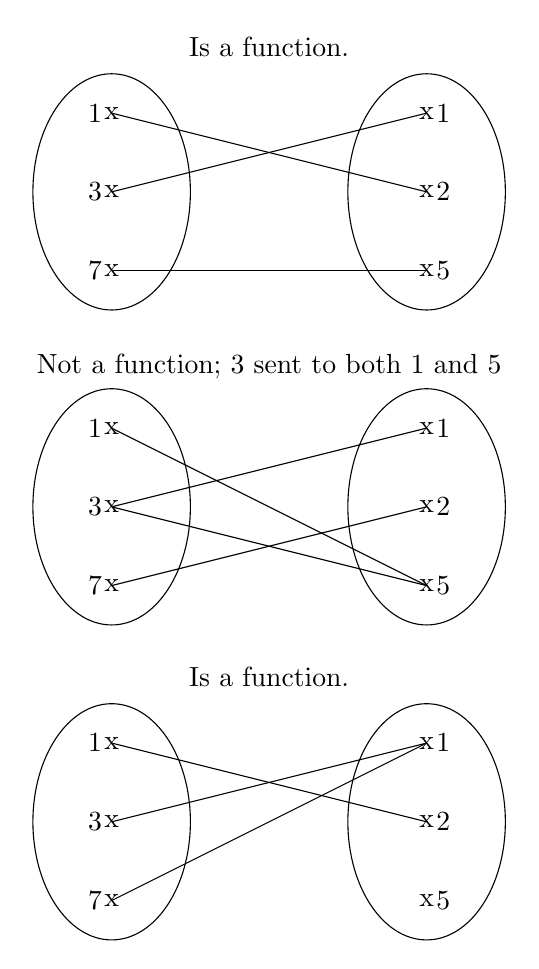
\begin{tikzpicture}	
					\begin{scope}
						\draw (0, 1.6) node[above] {Is a function.};
						\coordinate (A1) at (-2, 1);
						\coordinate (A2) at (-2, 0);
						\coordinate (A3) at (-2, -1);
					
						\draw (A1) node{x} node[left]{1};
						\draw (A2) node{x} node[left]{3};
						\draw (A3) node{x} node[left]{7};
						
						\coordinate (B1) at (2, 1);
						\coordinate (B2) at (2, 0);
						\coordinate (B3) at (2, -1);
						
						\draw (B1) node{x} node[right]{1};
						\draw (B2) node{x} node[right]{2};
						\draw (B3) node{x} node[right]{5};
						
						\draw (-2, 0) circle [x radius=1, y radius=1.5];
						\draw (2, 0) circle [x radius=1, y radius=1.5];
						
						\draw (A1) -- (B2);
						\draw (A2) -- (B1);
						\draw (A3) -- (B3);
					\end{scope}
					
					\begin{scope}[yshift=-4cm]
						\draw (0, 1.5) node[above] {Not a function; 3 sent to both 1 and 5};
						\coordinate (A1) at (-2, 1);
						\coordinate (A2) at (-2, 0);
						\coordinate (A3) at (-2, -1);
					
						\draw (A1) node{x} node[left]{1};
						\draw (A2) node{x} node[left]{3};
						\draw (A3) node{x} node[left]{7};
						
						\coordinate (B1) at (2, 1);
						\coordinate (B2) at (2, 0);
						\coordinate (B3) at (2, -1);
						
						\draw (B1) node{x} node[right]{1};
						\draw (B2) node{x} node[right]{2};
						\draw (B3) node{x} node[right]{5};
						
						\draw (-2, 0) circle [x radius=1, y radius=1.5];
						\draw (2, 0) circle [x radius=1, y radius=1.5];
						
						\draw (A1) -- (B3);
						\draw (A2) -- (B1);
						\draw (A2) -- (B3);
						\draw (A3) -- (B2);
					\end{scope}
					
					\begin{scope}[yshift=-8cm]
						\draw (0, 1.6) node[above] {Is a function.};
						\coordinate (A1) at (-2, 1);
						\coordinate (A2) at (-2, 0);
						\coordinate (A3) at (-2, -1);
										
						\draw (A1) node{x} node[left]{1};
						\draw (A2) node{x} node[left]{3};
						\draw (A3) node{x} node[left]{7};
										
						\coordinate (B1) at (2, 1);
						\coordinate (B2) at (2, 0);
						\coordinate (B3) at (2, -1);
										
						\draw (B1) node{x} node[right]{1};
						\draw (B2) node{x} node[right]{2};
						\draw (B3) node{x} node[right]{5};
										
						\draw (-2, 0) circle [x radius=1, y radius=1.5];
						\draw (2, 0) circle [x radius=1, y radius=1.5];
										
						\draw (A1) -- (B2);
						\draw (A2) -- (B1);
						\draw (A3) -- (B1);
					\end{scope}
				\end{tikzpicture}
			\end{figure}
			\item $A=B=\mathbb{R} \hspace{10mm} F:\mathbb{R} \rightarrow \mathbb{R}$ given by $f(x)=x$ is called the identity function.
		\end{enumerate}
		\item[Definition:] Let $A, B$ be sets and let $f: A \rightarrow B$ be a function. The \underline{range} of $f$ denoted by $f(A)$ if the subset of $B$ defined by $f(A) = \{y \in B \mid \exists x \in A$ s.t. $f(x)=y \}$.
		\item[Definition:] Let $A$ be a set. A \underline{Boolean function} on $A$ is a function $F:A \rightarrow \{T, F\}$ which has $A$ as its domain and the set of truth values $\{T, F\}$ as is codomain. $f:A \rightarrow \{T, F\}$ thus assigns truth values to the elements of $A$.
	\end{description}
	Function are often represented by graphs. If $f:A \rightarrow B$ is a function, the \underline{graph} of $f$ denoted $\Gamma (f)$ is the subset of the Cartesian product $A \times B$ given by $\{(x, f(x)) \mid x \in A \}.$
	\begin{description}
		\item[Q:] Is it possible to obtain every subset of $A \times B$ as the graph of some function?
		\item[A:] No! For $f:A \rightarrow B$ to be a function $\forall x ]in A \exists! y \in B$ s.t. $f(x)=y$, so for $\Gamma \subseteq A \times B$ to be the graph of some function, $\Gamma$ must satisfy that $\forall x \in A \exists! y \in B$ s.t. $(x, y) \in \Gamma$. Then we can define $f$ by letting $y = f(x)$.
	\end{description}
	
	\section{Composition of Functions}
	\begin{description}
		\item[Task:] Understand the natural operation that allows us to combine functions.
		\begin{figure}[h]
			\centering
			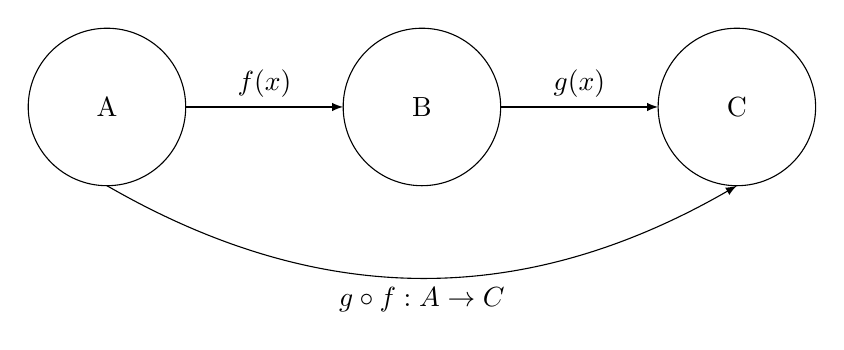
\begin{tikzpicture}
				\coordinate (A) at (-4, 0);
				\coordinate (B) at (0, 0);
				\coordinate (C) at (4, 0);
				
				\draw {(A) circle (1)} node{A};
				\draw {(B) circle (1)} node{B};
				\draw {(C) circle (1)} node{C};
				
				\draw [-latex](-3, 0) -- (-2, 0) node[above]{$f(x)$} -- (-1, 0);
				\draw [-latex](1, 0) -- (2, 0) node[above]{$g(x)$} -- (3, 0);
				\draw [-latex](-4, -1) to[bend right] node[below]{$g \circ f: A \rightarrow C$} (4, -1);
			\end{tikzpicture}
		\end{figure}
		\item[Example:] ~\\
		$f: \mathbb{R} \rightarrow \mathbb{R} \hspace{10mm} f(x) = 2x$ \\
		$g: \mathbb{R} \rightarrow \mathbb{R} \hspace{10mm} cos \: x$ \\
		$g \circ f(x) = g(f(x)) = g(2x = cos(2x))$ \\
		$f \circ g(x) = f(g(x)) = f(cos \: x) = 2(cos \: x) = 2 cos \: x$
	\end{description}
	
	\section{Inverting Functions}
	\begin{description}
		\item[Task:] Figure out which properties a function has to satisfy so that its action can be undone, \textbf{i.e.} when we can define an inverse to the original function.
	\end{description}
	Given $f: A \rightarrow B$, want $f^{-1}: B \rightarrow A$ s.t. $f^{-1} \circ f: A \rightarrow A$ is the identity $f^{-1} \circ f(x) = f^{-1}(f(x)) = x$ \\
	$A \overset{f}{\rightarrow} B \overset{f^{-1}}{\rightarrow} A$ \\
	It turns out $f$ has to satisfy two properties for $f^{-1}$ to exist.
	\begin{enumerate}
		\item Injective
		\item Surjective
	\end{enumerate}
	\begin{description}
		\item[Definition:] A function $f: A \rightarrow B$ is called \underline{injective} or an injection (sometimes called one to one) if $f(x)=f(y) \Rightarrow x=y$
		\item[Examples:] ~\\
		$\sin{x}: [0, \frac{\pi}{2}] \rightarrow \mathbb{R}$ is injective \\
		$\sin{x}: \mathbb{R} \rightarrow \mathbb{R}$ is not injective because $\sin{x} = \sin{\pi} = 0$
		\item[Definition:] A function $f: A \rightarrow B$ is called \underline{surjective} or a surjection (sometimes called onto) if $\forall z \in B \exists x \in A$ s.t. $f(x) = z$.
		\item[Remark:] $f$ assigns a value to each element of $A$ by its definition as a function, but it is not required to cover all of $B$. $f$ is surjective if its range is all of $B$.
		\item[Examples:] ~\\
		$\sin{x}: \mathbb{R} \rightarrow [-1, 1]$ is surjective \\
		$\sin{x}: \mathbb{R} \rightarrow \mathbb{R}$ is not surjective since $\nexists x \in \mathbb{R}$ s.t. $\sin{x} = 2$. We know $| \sin{x} | \leq 1 \forall x \in \mathbb{R}$
		\item[Definition:] A function $f:A \rightarrow B$ is called \underline{bijective} or a bijection if $f$ is \underline{both} injective and surjective.
		\item[Example:] $f: \mathbb{R} \rightarrow \mathbb{R} \hspace{10mm} f(x) = 2x+1$ is bijective.
		\begin{itemize}
			\item Check injectivity $f(x_1) = f(x_2) \Rightarrow 2x_1 + 1 = 2x_2 + 1 \Leftrightarrow 2x_1 = 2x_2 \Leftrightarrow x_1 = x_2$ as needed.
			\item Check surjectivity $\forall z \in \mathbb{R}. f(x) = z$ means $2x+1=z$. \\
			Solve for $x$: $2x=z-1 \Rightarrow x = \frac{z-1}{2} \in \mathbb{R} \Rightarrow f$ is surjective.
		\end{itemize}
		\item[Remark:] All bijective functions have inverses because we can define the inverse of a bijection and it will be a function:
		\begin{itemize}
			\item Surjectivity ensures $f_{-1}$ assigns an element to every element of $B$ (its domain).
			\item Injectivity ensures $f_{-1}$ assigns to each elements of $B$ \underline{one and only one} elements of $A$.
		\end{itemize}
		\item[Conclusion:] $f:A \rightarrow B$ bijective $\Rightarrow f_{-1}$ exists, \textbf{i.e.} $f_{-1} $ is a function. It turns out (reverse the arguments above) that $f_{-1}$ exists $\Rightarrow f:A \rightarrow B$ is bijective. \\
		Altogether we get the following theorem:
		\item[Theorem:] Let $f:A \rightarrow B$ be a function. $f_{-1}$ exists $\Leftrightarrow f:A \rightarrow B$ is bijective.
		\item[Q:] How do we find the inverse function $f_{-1}$ given $f: A \rightarrow B$?
		\item[A:] If $f(x)=y$, solve for $x$ as a function of $y$ since $f_{-1}(f(x))=f_{-1}(y)=x$ s $f_{-1} \circ f$ is the identity.
		\item[Example:] $f(x)=2x+1=y$. Solce for $x$ in terms of $y$. \\
		$f: \mathbb{R} \rightarrow \mathbb{R}$ \\
		$2x = y-1 \hspace{10mm} x = \frac{y-1}{2}$
	\end{description}
	
	\section{Functions Defined on Finite Sets}
	\begin{description}
		\item[Task:] Derive conclusions about a function given the number of elements of the domain and codomain if finite; understand the pigeonhole principle.
		\item[Proposition:] Let $A, B$ be sets and let $f:A \rightarrow B$ be a function. Assume $A$ is finite. Then $f$ is injective $\Leftrightarrow f(A)$ has the same number of elements as $A$.
		\item[Proof:]
		\item $A$ is finite so we can write it as $A = \{a_1, a_2, ..., a_p\}$ for some $p$. Then $f(A) = \{f(a_1), f(a_2), ..., f(a_p)\} \subseteq B$. A priori, some $f(a_i)$ might be the same as some $f(a_j)$. However, $f$ injective $\Leftrightarrow f(a_i) \neq f(a_j)$ whenever $i \neq j \Leftrightarrow f(A)$ has example $p$ elements just like $A$.
		\item[qed]
		\item[Corollary 1] Let $A, B$ be finite sets such that $\#(A) = \#(B)$. Let $f: A \rightarrow B$ be a function. $f$ is injective $\Leftrightarrow f$ is bijective.
		\item[Proof:]
		\item $\Rightarrow$ Suppose $f:A \rightarrow B$ is injective. Since $A$ is finite, by the previous proposition, $f(A)$ has the same number of elements as $A$, but $f(A) \subseteq B$ and $B$ has the same number of elements as $A \Rightarrow \#(A) = \#(f(A)) = \#(B)$, which means $f(A) - B$, \textbf{i.e.} $f$ is also surjective $\Rightarrow f$ is bijective.
		\item $\Leftarrow f$ is bijective $\Leftarrow f$ is injective.
		\item[qed]
		\item[Corollary 2 (The Pigeonhole Principle)] Let $A, B$ be finite sets. If $\#(B) < \#(A)$, and let $f:A \rightarrow B$ be a function. $\exists a, a' \in A$ where $ a \neq a'. f(a) = f(a')$
		\item[Remark:] The name pigeonhole principle is due to Paul Erd\"{o}s and Richard Rado. Before is was known as the principle of the drawers of Dirichlet. It has a simple statement, but it's a very powerful result in both mathematics and computer science.
		\item[Proof:] Since $f(A) \subseteq B$ and $\#(B) < \#(A), f(A)$ cannot hve as many elements as $A$, so by the proposition, $f$ cannot be injective, \textbf{i.e.} $\exists a, a' \in A$ where $a \neq a'$ (\textbf{i.e.} distinct elements) s.t. $f(a) = f(a')$
		\item[qed]
		\item[Examples:]
		\begin{enumerate}
			\item[]
			\item You have 8 friends. At least two of them were born the same day of the week. \#(days of the week) $= 7 < 8$.
			\item A family of five fives each other presents for Christmas. There are 12 presents under the tree. We conclude at least one person for three presents or more.
			\item In a list of 30 words in English, at least two will begin with the same letter. \#(Letter in the English alphabet) = 26 < 30.
		\end{enumerate}
	\end{description}
	
	\subsection{Behaviour of Functions on Infinite Sets}
	Let $A$ be a set and $f:A \rightarrow A$ be a function. If $A$ is finite , the corollary 1 tells us $f$ injective $\Leftrightarrow f$ bijective. What if $A$ is not finite?
	
	\subsubsection{Hilbert's Hotel problem (jazzier name: Hilbert's paradox of the Grand Hotel)}
	A fully occupied hotel with infinitely many rooms can always accommodate an additional guest as follows: The person in Room 1 removes to Room 2. The person in Room 2 moves to Room 3 and so on, \textbf{i.e.} if the rooms at $x_1, x_2, x_3...$ define the function $f(x_1)=x_2, f(x_2)=x_3, ..., f(x_m) = x_{m+1}$.
	
	\begin{description}
		\item[Claim:] As defined $f$ is injective but not surjective (hence not bijective!). Let $H = \{x_1, x_2,...\}$ the hotel consisting of infinitely many rooms. $f: H \rightarrow H$ is given by $f(x_n) = f(x_{n+1})$. $f(H) = H \backslash \{x_1\}$. We cn use this idea to prove:
		\item[Proposition:] A set $A$ is finite $\Leftrightarrow \forall f:A \rightarrow A$ an injective function is also bijective.
		\item[Proof:] If the set $X$ is finite then it follows immediately that every injective function $f:X \rightarrow X$ is bijective. \\
		Suppose that the set $X$ is infinite. Then there exists some infinite sequence $x_1, x_2, x_3, ...$ of distinct elements of $X$ (where an element of $X$ occurs at most once in this list). Then there exists a function $f:X \rightarrow X$ defined such that $f(x_n) = x_{n+1}$ for all positive integers of $n$, and $f(x) = x$ for all elements of $x$ of $X$. If $x$ is not a member of the infinite sequence $x_1, x_2, x_3, ...$ then the only elements of $X$ that gets mapped to $x$ is the element $x$ itself; if $x = x_n$, where $x>1$, then the only element of $X$ gets mapped to $x$. It follows that the function $f$ is injective. However it is not surjective, since $x_1$ does not belong to the range of the function. This function $f$ is thus an example of a function from the set $X$ to itself which is injective but not bijective.
	\end{description}
	
	\section{Mathematical Induction}
	\begin{description}
		\item[Task:] Understand how to construct a proof using mathematical induction.
	\end{description}
	$\mathbb{N} = \{0, 1, 2, ...\}$ set of natural numbers. \\
	Recall that $\mathbb{N}$ is constructed using 2 axioms:
	\begin{enumerate}
		\item $0 \in \mathbb{N}$
		\item If $n \in \mathbb{N}$, then $n+1 \in \mathbb{N}$
	\end{enumerate}
	
	\begin{description}
		\item[Remarks:]
		\begin{enumerate}
			\item[]
			\item This is exactly the process of counting.
			\item If we start at $1$, then we construct $\mathbb{N}* = \{1, 2, 3, 4, ...\} = \mathbb{N} \backslash \{0\}$
		\end{enumerate}
		\item via the axioms
		\begin{enumerate}
			\item $1 \in \mathbb{N}*$
			\item if $n \in \mathbb{N}*$, then $n+1 \in \mathbb{N}*$
		\end{enumerate}
		\item $\mathbb{N}$ or $\mathbb{N}*$ is used for mathematical induction.
	\end{description}
	
	\subsection{Mathematical Induction Consists of Two Steps:}
	\begin{description}
		\item[Step 1] Prove statements $P(1)$ called \underline{the base case}.
		\item[Step 2] For any $n$, assume $P(n)$ and prove $P(n+1)$. This is called \underline{the inductive step}. In other words, step 2 proves the statement $\forall n P(n) \rightarrow P(n+1)$
		\item[Remark:] Step 2 is not just an implication but infinitely many! In logic notation, we have:
		\item[Step 1] $P(1)$
		\item[Step 2] $\forall n (P(n) \rightarrow P(n+1))$ \\
		Therefore, $\forall n P(n)$ \\
		Let's see how the argument proceeds:
		\begin{enumerate}
			\item $P(1)$ \hspace{10mm} Step 1 (base case)
			\item $P(1) \rightarrow P(2)$ \hspace{10mm} by Step 2 with $n=1$
			\item $P(2)$ \hspace{10mm} by 1 \& 2
			\item $P(2) \rightarrow P(3)$ \hspace{10mm} by Step 2 with $n=2$
			\item $P(3)$ \hspace{10mm} by 3 \& 4
			\item $P(3) \rightarrow P(4)$ \hspace{10mm} by Step 2 with $n=3$
			\item $P(4)$ \hspace{10mm} by 5 \& 6 \\
			\vdots
			\item $P(n)$ for any $n$. \\
			This is like a row of dominos: knocking over the first one in a row makes all the others fall. Another idea is climbing a ladder.
		\end{enumerate}
		\item[Examples:]
		\begin{enumerate}
			\item[]
			\item Prove $1+3+5+...+(2n-1) = n^2$ by induction.
			\begin{description}
				\item[Base Case:] Verify statement for $n=1$
				\item When $n=1$, $2n-1 = 2 \times 1 - 1 = 1^2$
				\item[Inductive Step:] Assume $P(n)$, \textbf{i.e.} $1+3+5+...+(2n-1)=n^2$ and seek to prove $P(n+1)$, \textbf{i.e.} the statement $1+3+5...+(2n-1+2(n+1)-1) = (n+1)^2$
				\item We start with LHS: $1+ \underset{n^2}{\underbrace{3+5+...+(2n-1)}}+(2(n+1)-1)=n^2+2n+2-1=n^2+2n+1=(n+1)^2$
			\end{description}
			\item Prove $1+2+3+ +n= \frac{n(n+1)}{2}$ by induction.
			\begin{description}
				\item [Base Case:] Verify statement for $n=1$
				\item When $n=1, 1= \frac{1\times (1+1)}{2}=\frac{1 \times 2}{2} = 1$
				\item[Inductive Step:] Assume $P(n)$, \textbf{i.e.} $1+2+3+...+n=\frac{n\times (n+1)}{2}$ and seek to prove $1+2+3+...+n= \frac{(n+1)(n+2)}{2}$
				\item $\underset{\frac{n(n+1)}{2}}{\underbrace{1+2+3+...+n}}+n+1 = \frac{n(n+1)}{2} + n + 1 = (n+1)(\frac{n}{2} + 1)=(n+1)\frac{n+2}{2} = \frac{(n+1)(n+2)}{2}$ as needed.
			\end{description}
		\end{enumerate}
		\item[Remarks:]
		\begin{enumerate}
			\item[]
			\item For some argument by induction, it might be necessary to assume not just $P(n)$ at the inductive step but also $P(1), P(2)P, ...m P(n-1)$. This is called \underline{strong induction}.
			\begin{description}
				\item[Base Case:] Prove $P(1)$
				\item[Inductive Step:] Assume $P(a), P(2), ..., P(n)$ and prove $P(n+1)$.
			\end{description}
			\item[] An example of result requiring the use of strong induction is the \underline{Fundamental Theorem of Arithmetic}: $\forall n \in \mathbb{N}, n \geq 2, n$ can be expressed as a product of one or more prime numbers.
			\item One has to be careful with argument involving induction. Here is an illustration why:
			\item[] \underline{Polya's argument that all horses are the same colour:}
			\begin{description}
				\item[Base Case:] $P(1)$ There is only one horse, sot hat has a colour.\item[Inductive Step] Assume any $n$ horses are the same colour.
				\item Consider a group of $n+1$ horses. Exclude the first horse and look at the other $n$. All of these are the same colour by our assumption. Now exclude the last horse. The remaining $n$ horses are the same colour by our assumption. Therefore, the first horse, the horses in the middle, and the last horse are all of the same colour. We have established the inductive step.
				\item[Q:] Where does the argument fail?
				\item[A:] For $n=2, P(2)$ is false because there are no middle horses to compare to.
			\end{description}
			item[] \underline{The Grand Hotel Cigar Mystery}
			\begin{description}
				\item[] Recall Hilbert's hotel - the grand Hotel. Suppose that the Grand Hotel does not allow smoking and no cigars may be taken into the hotel. In spite of the rules, the guest in Room 1 goes to Room 2 to get a cigar. The guest in Room 2 goes to Room 3 to get 2 cigars (one for him and one for the person in room 1), etc. In other words, guest in Room N goes to Room N+1 to get N cigars. They will each get back to their rooms, smoke one cigar, and give the result to the person in Room N-2.
				\item[Q:] Where is the fallacy?
				\item[A:] This is an induction argument without a base case. No cigars are allowed in the hotel so no guests have cigars. An induction cannot get off the ground without a base case.
			\end{description}
		\end{enumerate}
	\end{description}
	
	\section{Abstract Algebra}
	\begin{description}
		\item[Task:] Understand binary operators, semigroups, monoids, and groups as well as their properties.
	\end{description}
	
	\subsection{Binary Operations}
	\begin{description}
		\item[Definition:] Let $A$ be a set. A \underline{binary operation} $*$ on $A$ is an operation applied to any two elements $x, y \in A$ that yields on elements $x*y$ in $A$. In other words, $*$ us a binary operation on $A$ if $\forall x, y \in A, x*y \in A$.
		\item[Examples:]
		\begin{enumerate}
			\item[]
			\item $\mathbb{R}, +$ addition on $\mathbb{R}: \forall x, y \in \mathbb{R}, x+y \in \mathbb{R}$
			\item $\mathbb{R}, -$ subtraction on $\mathbb{R}: \forall x, y \in \mathbb{R}, x-y \in \mathbb{R}$
			\item $\mathbb{R}, \times$ multiplication on $\mathbb{R}: \forall x, y \in \mathbb{R}, x \times y \in \mathbb{R}$
			\item $\mathbb{R}, /$, division on $\mathbb{R}$ is \underline{NOT} a binary operation because $\forall x \in \mathbb{R} \exists o \in \mathbb{R}$ s.t. $\frac{x}{o}$ is undefined (not an element of $\mathbb{R}$)
		\end{enumerate}
		\item[Definition:] A binary operation $*$ on a set $A$ is called \underline{commutative} if $\forall x, y \in A, x*y=y*x$
		\item[Examples:]
		\begin{enumerate}
			\item[]
			\item $\mathbb{R}, +$ is commutative since $\forall x, y \in \mathbb{R}, x+y=y+x$
			\item $\mathbb{R}, \times$ is commutative since $\forall x, y \in \mathbb{R}, x \times y = y \times x$
			\item $\mathbb{R}, -$ is not commutative since $\forall x, y \in \mathbb{R}, x-y \neq y-x$ in general. $x-y=y-x$ only if $x=y$
			\item Let $Mn$ be the set of $n$ by $n$ matrices with entries in $\mathbb{R}$ and let $*$ be matrix multiplication. $\forall A, B \in Mn, A*B \in Mn$, so $*$ is a binary operation, but $AB \neq BA$ in general. Therefore $*$ is not commutative.
		\end{enumerate}
		\item[Definition:] A binary operation $*$ on a set $A$ is called \underline{associative} if $\forall x, y z (x*y)*z = x*(y*z)$
		\item[Examples:]
		\begin{enumerate}
			\item[]
			\item $\mathbb{R}, +$ is associative since $\forall x, y, z \in \mathbb{R}, (x+y)+z=x+(y+z)$
			\item $\mathbb{R}, \times$ is associative since $\forall x, y, z \in \mathbb{R}, (x \times y) \times z = x \times (y \times z)$
			\item Intersection $\cap$ on sets is associative since $\forall A, B, C$ sets $(A \cap B) \cap C = A \cap (B \cap C)$.
			\item Union $\cup$ on sets is associative since $\forall A, B, C$ sets $(A \cup B) \cup C = A \cup (B \cup C)$
			\item $\mathbb{R}, -$ is not associative since $(1-3)-5 = -2-5 =-7$ but $1-(3-5)=1-(-2)=1+2=3$
		\end{enumerate}
		\item[Remark:] When we are dealing with associative binary operations we can drop the parentheses, \textbf{i.e.} $(x*y)*z$ can be written $x*y*z$.
	\end{description}
	
	\subsection{Semigroups}
	\begin{description}
		\item[Definition:] A \underline{semigroup} is a set endowed with an associative binary operation. We denote the semigroup $(A, *)$
		\item[Examples:]
		\begin{enumerate}
			\item[]
			\item $(\mathbb{R}, +)$ and $(\mathbb{R}, -)$ are semigroups.
			\item Let $A$ be a set and let $P(A)$ be its power set. $(P(A), \cap)$ and $(P(A), \cup)$ are both semigorups.
			\item $(Mn, *)$, the set of $n\times n$ matrices with entries in $\mathbb{R}$ with the operation of matrix multiplication (which is associative $\rightarrow$ a bit gory to prove) forms a semigroup.
			\item[] Since $*$ is associative on a semigroup, we can define $a^n:$\\
			$a^1 = a$ \\
			$a^2 = a*a$\\
			$a^3 = a*a*a$\\
			\vdots \\
			Recursively, $a^1=1$ and $a^n=a*a^{n-1}, \forall n > 1$
			\item[\textbf{NB:}] In $(\mathbb{R}, \times), \forall a \in \mathbb{R}, a^n = \underset{n\: times}{\underbrace{a \times a \times ... \times a}}$, whereas in $(\mathbb{R}, +), \forall a \in \mathbb{R}, a^n = \underset{n\: times}{\underbrace{a + a + ... + a}}=na$. Be careful what $*$ stands for!
		\end{enumerate}
		\item[Theorem:] Let $(A, *)$ be a semigroup. $\forall a \in A, a^m * a^n = a^{m+n}, \forall m, n \in \mathbb{N*}$.
		\begin{description}
			\item[Proof:] By induction on $m$.
			\item[Base Case:] $m=1 \hspace{10mm} a^1*a^n= a*a^n =a*{1+n}$
			\item[Inductive Step:] Assume the result is true for $m=p$, \textbf{i.e.} $a^p*a^n = a^{p+n}$ and seek to prove that $a^{p+1}*a^n=a^{p+1+n}$
			\item $a^p+1*a^n = (a*a^p)*a^n = a*(a^p*a*n) = a*a^{p+n} =a^{p+1+n}$
		\end{description}
		\item[Theorem:] Let$(A, *)$ be a semigroup. $\forall a \in A, (a^m)^n = a^{mn}, \forall m, n \in \mathbb{N}*$
		\begin{description}
			\item[Proof:] By induction on $n$.
			\item[Base Case:] $n=1 \hspace{10mm} (a^m)^1 = a^m = a^{m \times 1}$
			\item[Inductive Step:] Assume the result if true for $n=p$, \textbf{i.e.} $(a^m)^p = a^{mp}$ and seek to prove that $(a^m)^{p+1}=a^{m(p+1)}$
			\item $(a^m)^{p+1} = (a^m)^p * a^m = a^{mp} * a^m = a^{mp+m} = a^{m(p+1)}$
		\end{description}
	\end{description}
	
	\subsubsection{General Associative Law}
	Let $(A, *)$ be a semigroup. $\forall a_1, ..., a_s \in A, a_1 * a_2 * ... * a_s$ has the same value regardless of how the product is bracketed.
	\begin{description}
		\item[Proof] Use associativity of $*$.
		\item[qed]
		\item[NB:] Unless $(A, *)$ has a commutative binary operation, $a_1 * a_2 * ... * a_s$ does depend on the \underline{ORDER} in which the $a_j's$ appearin $a_1 * a_2 * ... * a_s$
	\end{description}
	
	\subsubsection{Identity Elements}
	\begin{description}
		\item[Definition:] Let $(A, *)$ be a semigroup. An element $e \in A$ is called an identity element for the binary operation $*$ if $e*x = x*e = x, \forall x \in A$.
		\item[Examples:]
		\begin{enumerate}
			\item[]
			\item $(\mathbb{R}, +)$ has 0 as the identity element.
			\item $(\mathbb{R}, \times)$ has 1 as the identity element.
			\item Given a set $A, (P(A), \cup)$ has $\emptyset$ (the empty set) as its identity elements, whereas $(P(A), \cap)$ does \underline{NOT} have an identity element.
			\item $(Mn, *)$ has $In$, the identity matrix as its identity element.
		\end{enumerate}
		\item[Theorem] A binary operation on a set cannot have more than one identity elements, \textbf{i.e.} if an identity element exists, then it is unique.
		\begin{description}
			\item[Proof:] Assume not (proof by contradiction). Let $e$ and $e'$ both be identity elements for a binary operation on a set $A$. $e=e*e'=e'$
			\item[qed]
		\end{description}
	\end{description}
	
	\subsection{Monoids}
	\begin{description}
		\item[Definition:] A \underline{monoid} is a set $A$ endowed with an associative binary operation $*$ that has an identity element $e$. In other words, a monoid is a semigroup $(A, *)$ where $*$ has an identity element $e$.
		\item[Definition:] A monoid $(A, *)$ is called \underline{commutative} (or \underline{Abelian}) if the binary operation $*$ is commutative.
		\item[Example:]
		\begin{enumerate}
			\item[]
			\item $(\mathbb{R}, +)$ is a commutative monoid with $e=o$.
			\item $(\mathbb{R}, \times)$ is a commutative monoid with $e=1$.
			\item Given a set $A$, $(P(A), \cup)$ is a commutative monoid with $e = \emptyset$.
			\item $(M,n *)$ is a monoid since $e=In$, but it is not commutative since matrix multiplication is not commutative.
			\item $(\mathbb{N}, +)$ is a commutative monoid with $e=o$, whereas $(\mathbb{N}*, +)$ is merely a semigroup (recall $\mathbb{N}* = \mathbb{N} \backslash\{0\}$)
		\end{enumerate}
		\item[Theorem:] Let $(A, *)$ be a monoid and let $a \in A$. Then $a^m * a^n = a^{m+n}, \forall m, n \in \mathbb{N}$
		\begin{description}
			\item[Remark:] Recall that we proved this theorem for semigroups if $m, n \in \mathbb{N}*$. We now need to extend that result.
			\item[Proof:] A monoid is a semigroup $\implies \forall a \in A, a^m * a^n = a^{m+n}$ whenever $m, n \in \mathbb{N}*$, \textbf{i.e.} $m > 0$ and $n > 0$. Now let $m = 0$. $a^m * a^n = a^0 * a^n = e * a^n = a^n = a^{0+n}$ \\
			If $n=0, a^m * a^n = a^m * a^0 = a^m* e = a^m = a^{m+0}$
			\item[qed]
		\end{description}
		\item[Theorem:] Let $A, *)$ be a monoid, $\forall a \in A \forall m, n \in \mathbb{N}, (a^m)^n = a^{mn}$
		\begin{description}
			\item[Remark:] Once again, we had this result for semigroups when $m>0$ and $n > 0$
			\item[Proof:] By the remark, we only need to prove the result when $m=0$ or $n=0$. If $m=0, (a^0)^n = (e)^n = e = a^0 = a^{0\times n}$. If $n=0$ then $(a^m)^0 = e = a^0 = a^{0 \times m}$
		\end{description}
	\end{description}
	
	\section{Inverses}
	\begin{description}
		\item[Task:] Understand what an inverse is and what formal properties it satisfies.
		\item[Definition:] Let $(A, *)$ be a monoid with identity element $e$ and let $a \in A$. An element $y$ of $A$ is called the \underline{inverse} of $x$ if $x*y = y*x = e$. If an element $a \in A$ has an inverse, then $a$ is called \underline{invertible}.
		\item[Examples:]
		\begin{enumerate}
			\item[]
			\item $(\mathbb{R}, +)$ has identity element 0. $\forall x \in \mathbb{R}, (-x)$ is the inverse of $x$ since $x+(-x)=(-x)=x = 0$.
			\item $(\mathbb{R}, \times)$ has identity element 1. $x \in \mathbb{R}$ is invertible only if $x \neq 0$. If $x \neq 0$, the inverse of $x$ is $\frac{1}{x}$ since $x \times \frac{1}{x} = \frac{1}{x} \times x =1$.
			\item $(Mn, *)$ the identity element is $In$. $A \in Mn$ is invertible if $det(A) \neq 0$. $A^{-1}$ the inverse is exactly the one you computed in linear algebra. If $det(a) = 0, A$ is \underline{NOT} invertible.
			\item Given a set $A, (P(A), \cup)$ has $\emptyset$ as its identity element of all the elements of $P(A)$ only $\emptyset$ is invertible and has itself asits inverse: $\emptyset \cup \emptyset= \emptyset \cup \emptyset = \emptyset$
		\end{enumerate}
		\item[Theorem:] Let $(A, *)$ be a monoid. If $a \in A$ has an inverse, then that inverse is unique.
		\begin{description}
			\item[Proof:] By contradiction: Assume not, then $\exists a \in A$ s.t. both $b$ and $c$ in $A$ are its inverses, \textbf{i.e.} $a*b = b*a = e$, the identity element of $(A, *)$ and $a*c = c*a = e$ and $b \neq c$, then $b = b*e=b*(a*c)=(b*a)*c=e*c=c$.
			\item[qed]
		\end{description}
		\item Since every invertible element of $a$ for $(A, *)$ a monoid has a unique inverse, we can denote the inverse by the more standard notation $a^{-1}$.
		\item Next, we need to understand inverses of elements obtained via the binary operation:
		\item[Theorem:] Let $(A, *)$ be a monoid and let $a, b$ be invertible elements of $A$. $a*b$ is also invertible and $a*b^{-1} = b^{-1}*a^{-1}$.
		\begin{description}
			\item[Remark:] You might remember this formula from linear algebra when you looked at the inverse of a product of matrices $AB$.
			\item[Proof:] Let $e$ be the identity element of $(A, *)  a*a^{-1} = a^{-1}*a = e$ and $b * b^{-1} = b^{-1}*b = e$. We would like to show $b^{-1} * a*{-1}$ is the inverse of $a*b$ by computing $(a*b)*(b^{-1} * a^{-1})$ and $(b^{-1} * a^{-1}) * (a*b)$ and showing both are $e$.
			\item $(a*b)*(a^{-1}*b^{-1}) = a*(b*b^{-1})*a^{-1} = a*e*a^{-1} = a*a^{-1} = e$
			\item $(b^{-1}*a^{-1})*(a*b) = b^{-1}*(a^{-1}*a)*b = b^{-1}*e*b = (b^{-1}*e)*b = b^{-1}*b=e$
			\item Thus $b^{-1}*a^{-1}$ satisfies the conditions needed for it to be the inverse of $a*b$.Since an inverse of unique, $a*b$ is invertible and $b^{-1}*a^{-1}$.
		\end{description}
		\item[Theorem:] Let $(A, *)$ be a monoid, and let $a, b \in A$. Let $x \in A$ be invertible. $a=b*x \Leftrightarrow b = a*x^{-1}$. Similarly, $a=x*b \Leftrightarrow b = x^{-1}*a$
		\begin{description}
			\item[Proof:] Let $e$ be the identity element of $(A, *)$.
			\item First $a=b*x \Leftrightarrow b = a*x^{-1}$:
			\item $\Rightarrow$ Assume $a=b*x. a*x^{-1} = (b*x)*x^{-1} = b*{x*x^{-1}} = b*e = b$ as needed.
			\item $\Leftarrow$ Assume $b=a*x^{-1}$. Then $b*x=(a*x^{-1})=a*(x^{-1}*x)=a*e=1$ as needed.
			\item Apply the same type of argument to show $a=x*b \Leftrightarrow b=x^{-1}*a$.
			\item[qed]
		\end{description}
		\item Let $(A, *)$ be a monoid. We can now make sense of $a^n$ for $n \in \mathbb{Z}, n < -$ for every $n \in A$ invertible. Since $n$ is a negative integer, $\exists p \in \mathbb{N}$ s.t. $n=-1$. Set $a^n = a^{-p}=(a^p)^{-1}$.
		\item[Theorem:] Let $(A, *)$ be a monoid and let $a \in A$ be invertible. Then $a^n * a^m = a^{m+n} \hspace{10mm} \forall m, n \in \mathbb{Z}$.
		\begin{description}
			\item[Proof:] When $m \geq 0 \land n \geq n$ we have already proven this result. The rest of the proof splits into cases.
			\item[Case 1:] $m=n \lor n = 0$
			\item If $m=0, n \in \mathbb{Z}, a^m * a^n = a^0 * a^n = e * a^n = a^n = a^{0+n}$ as needed.
			\item If $m \in \mathbb{Z}, n = 0, a^m * a^n = a^m * a^0 = a^m * e = a^m = a^{m+0}$ as needed.
			\item[Case 2:] $m < 0 \land n < 0$
			\item $m < 0 \Rightarrow \exists p \in \mathbb{N} \: s.t. \: p = -m. \: n<0 \Rightarrow \exists q \in \mathbb{N} \: s.t. \: q = -n.$
			\item $a^m = a^{-p} = (a^p)^{-1} \land a^n = a^{-q} = (a^q)^{-1}$
			\item $a^m * a^n = (a^p)^{-1} * (a^q)^{-1} = (a^q * a^p)^{-1} = (a^{p+q})^{-1} = a^{-(p+q)} = a^{-q-p} = a^{m+n} = a^{n+m}$
			\item[Case 3:] $m \land n$ have opposite signs.\\
			Without loss of generality, assume $m<0 \land n>0$ (the case $m>0 \land n<0$ is handled by the same argument). Since $m<0, \exists p \in \mathbb{N} \: s.t. \: p = -m.$ This case splits into two subcases:
			\begin{description}
				\item[Case 3.1:] $m+n \geq 0$
				\item Set $q = m+n$. Then $a^{m+n} = a^q = e*a^q = (a^p)^{-1} * a^p * a^q = (a^p)^{-1} * a^{p+q} = a^{-p} * a^{p+q} = a^m * a^{-m+m+n} = a^m * a^n$
				\item[Case 3.2:] $m+n < 0$
				\item Set $q = -(m+n) = -m-n \in \mathbb{N}^*$. Then $a^{m+n} = a^{-q} = (a^q)^{-1} * e = (a^q)^{-1} * (a^{-n} * a^n) = (a^q)^{-1} * (a^n)^{-1} *a^n = (a^n * a^q)^{-1} * a^n = (a^{n+p})^{-1} * a^n = (a^{n-m-n})^{-1} * a^n = (a^{-m})^{-1} * a^n = (a^p)^{-1} * a^n = a^m * a^n$
			\end{description}
		\end{description}
		\item[Theorem:] Let $(A, *)$ be a monoid, and let $a$ be an invertible element of $A$. $\forall m, n \in \mathbb{Z}, (a^m)^n = a^{mn}$.
		\begin{description}
			\item[Proof:] We consider 3 cases:
			\item[Case 1:] $n > 0$, \textbf{i.e.} $n \in \mathbb{N}^*. \: m \in \mathbb{Z}$ with no additional restrictions we proceed by induction on $m$.
			\begin{description}
				\item[Base Case:] $n=1 \hspace{10mm} (a^m)^1 = a^m = a^{m \times 1}$
				\item[Inductive Step:] We assume $(a^m)^n = a^{mn}$ and seek to prove $(a^m)^{n+1} = a^{m(n+1)}$. Start with $(a^m)^{n+1} = (a^m)^n * (a^m)^1 = a^{mn} * a^m = a^{mn+m} = a^{m(n+1)}$
			\end{description}
			\item[Case 2:] $n=0$; no restriction on $m \in \mathbb{Z}$
			\item $(a^m)^n = (a^m)^0 = e = a^0 = a^{m \times 0} = a^{mn}$
			\item[Case 3:] $n < 0$; no restriction on $m \in \mathbb{Z}$.
			\item Since $n < 0, \exists p \in \mathbb{N} \: s.t. \: p = -n$. By case 1, $(a^m)^p = a^{mp}$
			\item $(a^m)^n = (a^m)^{-p} = ((a^m)^p)^{-1} = (a^{mp})^{-1} = a^{-mp} = ^{m(-p)} = a^{mn}$
		\end{description}
	\end{description}
	
	\subsection{Groups}
	A motion formally defined in the 1870's even though theorems about groups proven as early as a century before that.
	\begin{description}
		\item[Definition:] A group os a monoid in which every element is invertible. In other words, a group is a set $A$ endowed with a binary operation $*$ satisfying the following properties:
		\begin{enumerate}
			\item $*$ is associative, \textbf{i.e.} $\forall x, y, z \in A, (x*y)*z = x*(y*z)$
			\item There exists an identity element $e \in A$, \textbf{i.e.} $\exists e \in A \: s.t. \: \forall a \in A, a*e = e*a = a$
			\item Every element of $A$ in invertible, \textbf{i.e.} $\forall a \in A \exists a^{-1} \in A \: s.t. \: a * a^{-1} = a^{-1} * a = e$
		\end{enumerate}
		\item[Notation for Groups:] $(A, *) \lor (\underset{set}{\underbrace{A}}, \underset{operation}{\underbrace{*}}, \underset{identity}{\underbrace{e}})$
		\item[Remark:] Closure under the operation $*$ is \underline{implicit} in the definition \textbf{i.e.} $\forall a, b \in A, a * b \in A$
		\item[Definition:] A group $(A, *, e)$ is called \underline{commutative} or \underline{Abelian} if its operation $*$ is commutative.
		\item[Examples:]
		\begin{enumerate}
			\item[]
			\item $(\mathbb{R}, +, 0)$ is an Abelian group.
			\item[] $-x$ is the inverse of $x, \forall x \in \mathbb{R}$
			\item $(\mathbb{Q}^*, \times, 1) \hspace{10mm} \mathbb{Q}^* = \mathbb{Q}^*\backslash\{0\} \hspace{10mm} (\mathbb{Q}^*, \times, 1)$ is Abelian
			\item[] $\forall q \in \mathbb{Q}^*, q^{-1} = \frac{1}{q}$ is the inverse.
			\item $(\mathbb{R}^3, +, 0)$ vectors in $\mathbb{R}^3$ with vector addition forms an Abelian group.
			\item[] $(x, y, z)+(x', y', z') = (x+x', y+y', z+z')$ vector addition.
			\item[] $0 = (0, 0, 0)$ is the identity. \hspace{10mm} $(-x, -y, -z) = - (x, y, z)$ is the inverse of $(x, y, z)$.
			\item $($\~{M}$m, *, In)$ $n\times n$ invertible matrices with real coefficients under matrix multiplication with $In$ as the identity elements forms a group which is \underline{NOT} Abelian.
			\item Set $A = \mathbb{Z}$ and recall the equivalence relation $x \equiv y$ mod $3$ \textbf{i.e.} $x \land y$ have te same remainder under the division by $3$. Recall that $\mathbb{Z} / N = \{0, 1, 2\}$, \textbf{i.e.} the set of equivalence classes under the partition determined by this equivalence relation. We denote $\mathbb{Z} / N \ \{0, 1, 2\} = \mathbb{Z}_3$
			\item[] Consider $(\mathbb{Z}_3, \oplus _3, 0)$ where $\oplus _3$ is the operation of addition modulo $3$, \textbf{i.e.} $1+0=1, 1+1=2, 1+2=3 \equiv 0$ mod $3$.
			\item[\textbf{Claim:}] $(\mathbb{Z}_3, \oplus _3, 0)$ is an Abelian group.
			\item[\textbf{Proof of Claim:}] Associativity of $\oplus _3$ follows from the associativity of $+$, addition of $\mathbb{Z}$. Clearly, $0$ is the identity (don't forget $0$ stands for all elements with remainder $0$ under division by $3$, \textbf{i.e.} $\{0, 3, -3, 6, -3, ...\}$). To compute inverses recall that $a \oplus _3 a^{-1} = 0, 0$ is the inverse of $0$ because $0+0=0$. $2$ is he inverse of $1$ because $1+2=3 \equiv 0$ mod $3$, and $1$ is the inverse of $2$ because $2+1=3 \equiv 0$ mod $3$. \\
			More generally, consider the equivalence relation on $\mathbb{Z}$ given by $x \equiv y$ mod $n$ for $n \geq 1. \mathbb{Z} / N = \{0, 1, ..., n-1\} = \mathbb{Z}_n$. All possible remainders under division by $n$ are the equivalence classes. Let $\oplus _n$ be addition mod $n$. By the same argument as above, $(\mathbb{Z}_n, \oplus _n, 0)$ is an Abelian group.
			\item[\textbf{Q:}] What is we consider multiplication mod $n$, \textbf{i.e.} $\otimes _n$. Is $(\mathbb{Z}_n, \otimes _n, 1)$ a group?
			\item[\textbf{A:}] No! $(\mathbb{Z}_n, \otimes _n, 1)$ is not even a monoid because $1 \otimes _n 0 = 0 \otimes _n 1 = 0$, so $1$ is not an identity element for $\otimes _n$ on $\mathbb{Z}_n$.
			\item[\textbf{Q:}] Can this be fixed?
			\item[\textbf{A:}] Troubleshoot how to get rid of 0. \\
			Consider $\mathbb{Z}_n^* = \mathbb{Z}_n \backslash \{0\} = \{1, 2, ..., n-1\}$ all non-zero elements in $\mathbb{Z}_n^*$. This eliminates 0 as an element, but can 0 arise any other way from the binary operation? It turns out the answer depends on $n$. If $n$ is not prime, say $n=6$, we get two divisors, \textbf{i.e.} elements that yield 0 when multiplied by \underline{precisely} the factors of $n$, for $n=6$, $\mathbb{Z}^*_6 = \{1, 2, 3, 4, 5\}$ \underline{but} $2 \otimes _6 3 = 6 \equiv 0$ mod $6$, so $2 \land 3$ are two divisors.
			\item[\textbf{Claim:}] If $n$ is prime, then $(\mathbb{Z}_n^*, \otimes _n, 1)$ is an Abelian group. \\
			Used in cryptology $\rightarrow$ you will see next semester. \\
			As an example, let us look at the multiplication table for $\mathbb{Z}_5^*$ to see the inverse of various elements: $\mathbb{Z}^*_5 = \mathbb{Z}_5 \backslash \{0\} = \{0, 1, 2, 3, 4,\} \backslash \{0\} - \{1, 2, 3, 4\}$
	
			\begin{center}
				\begin{tabular}[h!]{|c|cccc|rl}
					\cline{1-5}
					& 1 & 2 & 3 & 4\\ \cline{1-5}
					1 & 1 & 2 & 3 & 4 & \hspace{10mm} $1^{-1} = 1$ & $1 \otimes_5 1 = 1$ \\
					2 & 2 & 4 & 1 & 2 & \hspace{10mm} $2^{-1} = 3$ & $2 \otimes_5 3 = 6 \equiv 1$ mod $5$ \\
					3 & 3 & 1 & 4 & 2 & \hspace{10mm} $3^{-1} = 2$ & $3 \otimes_5 2 = 6 \equiv 1$ mod $5$ \\
					4 & 4 & 3 & 2 & 1 & \hspace{10mm} $4^{-1} = 1$ & $4 \otimes_5 4 = 16 \equiv 1$ mod $5$ \\
					\cline{1-5}
				\end{tabular}
			\end{center}
			The fact that $\mathbb{Z}^*_n, \otimes _n, 1$ is Abelian follows from the commutativity of multiplication on $\mathbb{Z}$.
			\item Let $(A, *, e)$ be any group and let $a \in A$. \\
			Consider $A' = \{a^m \mid m \in \mathbb{Z}\}$ all powers of $a$. It turns out $(A', *, e)$ is a group called the \underline{cyclic group} determined by $a$. $(A', *, e)$ is Abelian \underline{regardless} of whether the original group was Abelian or not because of the theorem we proved on powers of $a$: $\forall m, n \in \mathbb{Z} \hspace{10mm} a^m * a^n = a^{m+n} = a^{n+m} = a^n * a^m$. \\
			Cyclic groups come in two flavours: finite ($A'$ is a finite set) and infinite ($A'$ is an infinite set). \\
			For example, let $(A, *, e) = (\mathbb{Q}^*, , \times , 1)$ \\
			If $a=-1 \hspace{10mm} A' = \{(-1)^m \mid m \in \mathbb{Z}\} = \{-1, 1\}$ is finite. \\
			If $a=2 \hspace{10mm} A' = \{2^m \mid m \in \mathbb{Z}\} = \{1, 2, \frac{1}{2}, 4, \frac{1}{4}, ...\}$ is infinite.
		\end{enumerate}
	\end{description}
	
	\section{Homomorphisms and Isomorphisms}
	\begin{description}
		\item[Task:] Understand the most natural functions between objects in abstract algebra such as semigroups, monoids or groups.
		\item[Definition:] Let $(A, *)$ and $(B, *)$ ve vitg semigroups, monoids or groups. A function $f: A \rightarrow B$ is called a \underline{homomorphism} if $f(x * y) = f(x) * f(y) \: \forall x, y \in A$. In other words, if $f$ is a function that respects (behaves well with respect) to the binary operation.
		\item[Examples:]
		\begin{enumerate}
			\item[]
			\item Consider $(\mathbb{Z}, +, 0)$ and $(\mathbb{R}^*, \times, 1)$. \\
			Pick $a \in \mathbb{R}^*$, then $f(n) = a^n$ is a homomorphism between $(\mathbb{Z}, +, 0)$ and $(\mathbb{R}^*, \times, 1)$ because $(\mathbb{R}^*, \times, 1)$ is a group, and we proved for groups that $a^{m+n} = f(m+n) = a^m * a^n = f(m) * f(n) \hspace{10mm} \forall m, n \in \mathbb{Z}$.
			\item More generally, $\forall a \in A$ invertible, where $(A, *)$ is a monoid with identity element $e$, $f(n) = a^m$ gives a homomorphism between $(\mathbb{Z}, +, 0)$ and $(A', *, e)*$, where as before $A' = \{a^m \mid m \in \mathbb{Z}\} \subset A$. \\
			We get even better behaviour if we require $f:A \rightarrow B$ to be bijective.
		\end{enumerate}
		\item[Definition:] Let $(A, *)$ and $(B, *)$ both be semigroups, monoids or groups. A function $f:A \rightarrow B$ is called an isomorphism if  $f:A \rightarrow B$ is both bijective \underline{AND} a homomorphism.
		\item[Examples:]
		\begin{enumerate}
			\item[]
			\item Let $A' = \{2^m \mid m \in \mathbb{Z}\} = \{1, 2, \frac{1}{2}, 4, \frac{1}{4}, ...\}$ \\
			$f(m) = 2^m$ from $(\mathbb{Z}, +, 0)$ to $(A', \times, 1)$ is an isomorphism since $2^m \neq 2^n$ if $m \neq n$.
			\item Let $A' = \{(-1)^m \mid m \in \mathbb{Z} \} = \{-1, 1\}$ \\
			$f(m) = (-1)^m$ from $(\mathbb{Z}, +, 0)$ to $(A', \times, 1)$ is \underline{NOT} an isomorphism since it's not injective $(-1)^2 = (-1)^4 = 1$.
		\end{enumerate}
		\item[Theorem:] Let $(A, *)$ and $(B, *)$ both be semigroups, monoids or groups. The inverse $f^{-1}: B \rightarrow A$ of any isomorphism  $f: A \rightarrow B$ from $A$ to $B$ is itself an isomorphism.
		\item[Proof:] If $f: A \rightarrow B$ is an isomorphism $\Rightarrow f:A \rightarrow B$ is bijective $\Rightarrow f^{-1}:B \rightarrow A$ is bijective (proven when we discussed functions).
		\item To show $f^{-1} B \rightarrow A$ is a homomorphism, let $u, v \in B$. $\exists x, y \in A$ s.t. $x = f^{-1}(u)$ and $y = f^{-1}(v)$, but then $u = f(x)$ and $v = f(y)$.
		\item Since $f: A \rightarrow B$ is a homomorphism, $f(x * y) = f(x) * f(y) = u*v$. Then $f^{-1}(u*v) = f^{-1}(f(x*y)) = x*y = f^{-1}(u)*f^{-1}(v)$ as needed.
		\item[qed]
		\item[Definition:] Let $(A, *)$ and $(B, *)$ both be semigroups, monoids or groups. If $\exists f:A \rightarrow B$ an isomorphism betwen $A$ and $B$, then $(A, *)$ and $(B, *)$ are said to be isomorphic.
		\item[Remark:] "Ismorphic" comes from "iso" same + "morph\'{e}" form same abstract algebra structure on both $(A, *)$ and $(B, *)$ given to you in two different guises. As the French would say: "M\^{e}me Marie, autre chapeau" same Mary, different hat.
	\end{description}
	
	\section{Formal Languages}
	\begin{description}
		\item[Task:] Use what we learned about structues in abstract algebra in order to make sense of formal languages and grammars. \\
		Let $A$ be a finite set. When studying formal languages, we call $A$ an \underline{alphabet} and the elements of $A$ \underline{letters}.
		\item[Examples:]
		\begin{enumerate}
			\item[]
			\item $A = \{0, 1\}$ \hspace{10mm} binary digits
			\item $A = \{0, 1, 2, 3, 4, 5, 6, 7, 8, 9\}$ \hspace{10mm} decimal digits
			\item $A =$ {letters of the English alphabet}
		\end{enumerate}
		\item[Definition:] $\forall n \in \mathbb{N}^*$, we define a \underline{word} of length $n$ in the alphabet $A$ as being any string of the form $a_1, a_2, ..., a_n \: s.t. \: a_i \in A \hspace{5mm} \forall i, 1 \leq i \leq n$. Let $A^n$ be the set of all words of length $n$ over the alphabet $A$.
		\item[Remark:] There is a one-to-one correspondence between the string $a_1a_2...a_n$ and the ordered n-tuple $(a_1, a_2, ..., a_n) \in A^n = \underset{n \: times}{\underbrace{A \times ... \times A}}$ the Cartesian product of $n$ copies of $A$.
		\item[Definition:] Let $A^+ = \underset{n=1}{\overset{\infty}{\cup}} A^n = A^1 \cup A^2 \cup A^3 \cup ...$. $A^+$ is the set of all words of positive length over the alphabet $A$.
		\item[Examples:]
		\begin{enumerate}
			\item[]
			\item $A = \{0, 1\}, A^+$ is the set of all binary strings of finite length that is at least on, \textbf{i.e.} $0, 1, 01, 10, 00, 11,$ etc.
			\item If $A =$ {letters of the English alphabet}, then $A^+$ consists of all non-empty strings of finite lengths of letters from the English alphabet. \\
			It is useful to also have the empty for $\varepsilon$ in our set of strings. $\varepsilon$ has length 0. Define $A^0 = \{\varepsilon\}$ and then adjoin the empty word $\varepsilon$ to $A^+$. We get $A^* = \{\varepsilon\} \cup A^+ = A^0 \cup \underset{n=1}{\overset{\infty}{\cup}} A^n = \underset{n=0}{\overset{\infty}{\cup}} A^n$.
		\end{enumerate}
		\item[Notation:] We denote the length of a word $w$ by $\mid w \mid$. Next introduce an operation on $A^*$.
		\item[Definition:] Let $A$ be a finite set and let $w_1 \land w_2$ be words in $A^*$. $w_1 = a_1a_2...a_m \land w_2 = b_1b_2...b_n$. The \underline{concatenation} of $w_1 \land w_2$ is the word $w_1 \circ w_2$, where $w_1 \circ w_2 = a_1a_2...a_mb_1b_2...b_n$. Sometimes $w_1 \circ w_2$ is denoted as just $w_1w_2$. Note that $\mid w_1 \circ w_2 \mid = \mid w_1 \mid + \mid w_2 \mid$. \\
		Concatenation of words is:
		\begin{enumerate}
			\item associative
			\item \underline{NOT} commutative is $A$ has more than one element.
		\end{enumerate}
		\begin{description}
			\item[Proof of (1):] Let $w_1, w_2, w_3 \in A^*. w_1 = a_1a_2...a_m$ for some $m \in \mathbb{N}, w_2=b_1b_2...b_n$ for some $m \in \mathbb{N}$ and $w_3 = c_1c_2...c_p$ for some $p \in \mathbb{N}$. $w_1 \circ w_2) \circ w_3 = w_1 \circ (w_2 \circ w_3) = a_1a_2...a_mb_1b_2...b_nc_1c_2...c_p$.
			\item[qed]
			\item[Proof of (2):] Since $A$ has at least two elements, $\exists a, b \in A$ s.t. $a \neq b$.
			\item $a \circ b = ab \neq ba = b \circ a$.
			\item[qed]
		\end{description}
		\item $A^*$ is closed under the operation of concatenation $\Rightarrow$ concatenation is a binary operation of $A^*$ as $\forall w_1, w_2 \in \AA^*, w_1 \circ w_2 \in A^*$.
		\item[Theorem] Let $A$ be a finite set. $(A^*, \circ)$ is a monoid with identity element $\varepsilon$.
		\item[Proof:] Concatenation $\circ$ is an associative binary operation on $A^*$ as we showed above. Moreover, $\forall w \in A^*, \varepsilon \circ w = w \circ \varepsilon = w$, so $\varepsilon$ is the identity element of $A^*$.
		\item[qed]
		\item[Definition:] Let $A$ be a finite set. A \underline{language} over $A$ is a subset of $A^*$. A language $L$ over $A$ is called a \underline{formal language} is $\exists$ a finite set of rules of algorithm that generates exactly $L$, \textbf{i.e.} all words that belong to $L$ and no other words.
		\item[Theorem:] Let $A$ be a finite set.
		\begin{enumerate}
			\item If $L_1$ and $L_2$ are languages over $A, L_1 \cup L_2$ is a language over $A$.
			\item If $L_1$ and $L_2$ are languages over $A, L_1 \cap L_2$ is a language over $A$.
			\item If $L_1$ and $L_2$ are languages over $A$, the concatenation of $L_1 \land L_2$ given by $L_1 \circ L_2 = \{w_1 \circ w_2 \in A^* \mid w_1 \in L_1 \land w_2 \in L_2\}$ is a language over $A$.
			\item Let $L$ be a language over $A$. Define $L^1=L$ inductively for and $n\geq 1 \hspace{5mm} L^n = L \circ L^{n-1}. L^n$ is a language over $A$. Furthermore, $L^* = \{\varepsilon\} \cup L^! \cup L^2 \cup L^3 \cup ... = \underset{n=0}{\overset{\infty}{\cup}} L^n$ is a language over $A$.
		\end{enumerate}
		\item[Proof:] By definition, a language over $A$ is a subset of $A^*$. Therefore, if $L_1 \subseteq A^* \land L_2 \subseteq A^*$, then $L_1 \cup L_2 \subseteq A^* \land L_1 \cap L_2 \subseteq A^*. \forall w_1 \circ w_2 \in L_1 \circ L_2, w_1 \circ w_2 \in A^*$ becomes $w_1 \in A^n$ for some $n$ and $w_2 \in A^m$ for some $m$ so $w_1 \circ w_2 \in A^{m+n} \subseteq A^* = \underset{n=1}{\overset{\infty}{\cup}} A^n$.
		\item Applying the same reasoning inductively, we see that $L \subset A^* \Rightarrow L^* \subseteq A^*$ as $L^m \subseteq A^* \: \forall n \geq 0$.
		\item[qed]
		\item[Remark:] This theorem gives us a theoretic way of building languages, but we need a practical way. The practical way of building a language is through the notion of a grammar.
		\item[Definition:] A (formal) grammar is a set of production rules for strings in a language. \\
		To generate a language we use:
		\begin{enumerate}
			\item $A$ the set, which is the alphabet of the language.
			\item A start symbol $<$s$>$
			\item A set of production rules.
		\end{enumerate}
		\item[Example:] $A = \{0, 1\}$; start symbol $<$s$>$; 2 production rules given by:
		\begin{enumerate}
			\item $<$s$>$ $\rightarrow$ 0$<$s$>$1
			\item $<$s$>$ $\rightarrow$ 01
		\end{enumerate}
		Let's see what we generate: via rule 2 \hspace{5mm} $<$s$>$ $\rightarrow$ 01, so we get $<$s$>$ $\Rightarrow$ 01 \\
		Via rule 1 \hspace{5mm} $<$s$>$ $\rightarrow$ 0$<$s$>$1, then via rule 2, 0$<$s$>$1 $\rightarrow$ 0011. We write the process as $<$s$>$ $\rightarrow$ 0$<$s$>$1 $\Rightarrow$ 0011. \\
		Via rule 1, $<$s$>$ $\rightarrow$ 0$<$s$>$1, then via rule 1 again 0$<$s$>$1 $\rightarrow$ 00$<$s$>$11, then via rule 2, 00$<$s$>$11 $\rightarrow$ 000111. \\
		We got $<$s$>$ $\Rightarrow$ 0$<$s$>$1 $\Rightarrow$ 00$<$s$>$11 $\Rightarrow$ 000111. \\
		The language $L$ we generated thus consists of all strings of the form $0^m1^m$ ($m$ 0's followed by $m$ 1's) for all $m \geq 1, m \in \mathbb{N}$ \\
		We saw 2 types of strings that appeared in this process of generating $L$:
		\begin{enumerate}
			\item \underline{terminals}, \textbf{i.e.} the elements of $A$
			\item \underline{nonterminals}, \textbf{i.e.} strings that don't consist solely of 0's and 1's such as $<$s$>$, 0$<$s$>$1, 00$<$s$>$11, etc.
		\end{enumerate}
		The production rules then have the form:
		\begin{description}
			\item nonterminal $\rightarrow$ word over the alphabet V = {terminals, non-terminals}
			\item $<$T$>$ $\rightarrow$ w
		\end{description}
		In our notation, the set of nonterminals if $V \backslash A$, so $<$T$>\in V \backslash A \land w \in V^* - \underset{n=0}{\overset{\infty}{\cup}} V^n$. To the production rule $<$T$>\rightarrow w$. \\
		We can associate the ordered pair ($<$T$>, w) \in (V \backslash A) \times V^*$, so the set of production rules, which we will denote by $P$, is a subset of the Cartesian product $(V\backslash A) \times V^*$. \\
		Grammers come in two flavours:
		\begin{enumerate}
			\item \underline{Context-free grammars} where we can replace \underline{any} occurrence of $<$T$>$ by $w$ if $<$T$>\rightarrow w$ is one of our production rules.
			\item \underline{Context-sensitive grammars} only certain replacements of $<$T$>$ by $w$ are allowed, which are governed by the syntax of our language $L$.
		\end{enumerate}
		The example we have was of a context free grammar. We can now finally define context free grammars.
		\item[Definition:] A \underline{context free grammar} $(V, A, <$s$>P)$ consists o a finite set $V$, a subset $A$ of $V$, an element $<$s$>$ of $V \backslash A$, and a finite subset $P$ of the Cartesian product $V\backslash A \times V^*$.
		\item[Notation:] $(\underset{set\:of\:terminals\:and\:non\:terminals}{V}$, $\underset{set\:of\:terminals}{A}$, $\underset{start\:symbol}{{<}s{>}}$, $\underset{set\:of\:production\:rules}{P})$
		\item[Example:] $A = \{0, 1\}$; start symbol $<$s$>$; 3 production rules given by:
		\begin{enumerate}
			\item $<$s$>\rightarrow$ 0$<$s$>$1
			\item $<$s$>\rightarrow$ 01
			\item $<$s$>\rightarrow$ 0011
		\end{enumerate}
		We notice here that the word 0011 can be generated in 2 ways in this context free grammar:
		\begin{enumerate}
			\item[By rule 3,] $<$s$>\rightarrow$ 0011 so $<$s$>\Rightarrow$ 0011
			\item[] $\lor$
			\item[By rule 1,] $<$s$>\rightarrow$ 0$<$s$>$1 and by rule 2, 0$<$s$>$1 $\rightarrow$ 0011. Therefore, $<$s$>\Rightarrow$ 0$<$s$>$1 $\Rightarrow$ 0011.
		\end{enumerate}
		\item[Definition:] A grammar is called \underline{ambiguous} if it generates the same string in more than one way. \\
		Obviously, we prefer to have unambiguous grammars, else we waste computer operations. \\
		Next, we need to spell out how words \underline{relate} to each other in the production of our language via the grammar:
		\item[Definition:] Let $w'$ and $w"$ be words over the alphabet $V$ = {terminals, non-terminals}. We say that \underline{$w'$ directly yields $w"$} if $\exists$ words $u \land v$ over the alphabet $V$ and a production rule $<$T$>\rightarrow w$ of the grammar s.t. $w' = u<$T$>\land w" = uwv$, where either or both of the words $u$ and $v$ may be the empty word. \\
		In other words, $w'$ directly yields $w" \Leftrightarrow \exists$ production rule $<$T$>\rightarrow w$ in the grammar s.t. $w"$ may be obtained from $w'$ by replacing a simple occurrence of the nonterminal $<$T$>$ within the word $w'$ by the word $w$.
		\item[Notation:] $w'$ directly yields $w"$ is denoted by $w' \Rightarrow w"$
		\item[Definition:] Let $w' \land w"$ be words over the alphabet $V$. We say that $w'$ yields $w"$ if either $w'= w"$ or else $\exists$ words $w_0, w_1, ... w_n$ over the alphabet $V$ s.t. $w_0=w', w_n = w", w_{i-1} \Rightarrow w_i$ for all $i, 1 \leq i \leq n$. In other words, $w_0 \Rightarrow w_1 \Rightarrow w_2 \Rightarrow ... \Rightarrow w_n-1 \Rightarrow w_n$
		\item[Notation:] $w'$ yields $w"$ is denotes by $w' \overset{*}{\Rightarrow} w"$.
		\item[Definition:] Let $(V, A, <$s$>, P)$ be a context free grammar. The \underline{language} generated by this grammar is the subset $L$ or $A^*$ defined by $L = \{w \in A^* \mid <$s$>\overset{*}{\Rightarrow} w\}$ \\
		In other words, th language $L$ generated by a context free grammar $(V, A, <$s$>, P)$ consists of the set of all finite strings consisting entirely of terminals that may be obtained from the start symbol $<$s$>$ by applying a finite sequence of production rules of the grammar where the application of one production rule causes \underline{one and only one nonterminal} to be replaced by the string in $V^*$ corresponding of the right hand side of the production rule.
	\end{description}
	
	\subsection{Phrase Structure Grammars}
	\begin{description}
		\item[Definition:] A phrase structure grammar $(V, A <$s$>, P)$ consists of a finite set $V$, a subset $A$ of $V$, an element $<$s$>$ of $V \backslash A$, and a finite subset $P$ of $(V^* \backslash A^*) \times V^*$ \\
		In a context free grammar, the set of production rules $P \subset (V \backslash A) \times V^*$. \\
		In a phrase structure grammar, $P \subset (V^* \backslash A^*) \times V^*$. In other words, a production rule in a phrase structure grammar $r \rightarrow w$ has a left hand side $n$ that may contain more than one nonterminal. It is required to contain \underline{at least one} nonterminal. \\
		For example, if $A \{0, 1\}$ and $<$s$>$ is the start symbol in a phrase grammar grammar, 0$<$s$>$0$<$s$>$0 $\rightarrow$ 00010 would be an acceptable production rule in a phrase structure grammar but not in a context free grammar. \\
		The notions $w' \Rightarrow w"$ ($w'$ directly yields $w"$) and $w' \overset{*}{\Rightarrow} w"$ ($w'$ yields $w"$) are defined the same way as for context free grammars except that our production rules may, of course, be more general as we saw in the example above.
		\item[Definition:] Lt $(V, A <$s$>, P)$ be a phrase structure grammar. The language generated by this grammar is the subset $L$ or $A^*$ defined by $L \{w \in A^* \mid <$s $>\overset{*}{\Rightarrow} w \}$
		\item[Remark:] The term phrase structure grammars was introduced by Noam Chowsky.
		\item[Definition:] A lamguage $L$ generated by a context-free grammar is called a \underline{context-free language}.
	\end{description}
	We now want to understand a particularly important subclass of context free languages called regular languages.
	
	\section{Regular Languages}
	\begin{description}
		\item[Task:] Understand when a language is regular and how regular languages are produced. Understand basics of automata theory.
		\item[History:] The term \underline{regular languages} was introduced by Stephen Kleene in 1951. A more descriptive name is \underline{finite-state languages} as we will see that a language is regular $\Leftrightarrow$ it can be recognised by a finite state acceptor, which is a type of finite state machine. \\
		The definition of a regular language is very abstract, though. First, describe what operations the collection of regular languages is closed under: \\
		Let $A$ be a finite set, and let $A*$ be the set of all words over the alphabet $A$. The regular language over the alphabet $A$ consitute the smallest collection $C$ of subsets of $A*$ satisfying that:
		\begin{enumerate}
			\item All finite subsets of $A*$ belong to $C$.
			\item $C$ is closed under the Kleene start operation (if $M \subseteq A*$ is inside $C, \textbf{i.e.} M \subseteq C$, then $M* \subseteq C$)
			\item $C$ is closed under concatenation (if $M \subseteq A*, N \subseteq A*$ satisfy that $M \subseteq C \land N \subseteq C$, then $M \circ N \subseteq C$)
			\item $C$ is closed under union (if $M \subseteq A* \land N \subseteq A*$ satisfy that $M \subseteq C \land N \subseteq C$, then $M \cup N \subseteq C$)
		\end{enumerate}
		\item[Definition:] Let $A$ be a finite set, and let $A*$ be the set of words over the alphabet $A$. A subset $L$ of $A*$ is called a \underline{regular language} over the alphabet $A$ is $L = L_m$ for some finite sequence $L_1, L_2,..., L_m$ os subsets of $A*$ with the property that $\forall i, 1 \leq i \leq m, L_i$ satisfies one of the following:
		\begin{enumerate}
			\item $L_i$ is a finite set
			\item $L_i = L_j*$ for some $j, 1 \leq j \leq i$ (the Klenne star operation applied to one of the previous $L_j's$)
			\item $L_i = L_j \circ L_k$ for some $j, k$ such that $1 \leq j, k < i$ ($L_i$ is a concatenation of previous $L_j's$)
			\item $L_i = L_j \cup L_k$ for some $j, k$ such that $1 \leq k, j < i$ ($L_i$ is a union of previous $L_j's$)
		\end{enumerate}
		\item[Example 1:] Let $A = \{0, 1\}$. Let $L = \{0^M1^n \mid m, n \in \mathbb{N} \hspace{5mm} m \geq 0, n \geq 0 \}$ \\
		$L$ is a regular language. Note that $L$ consists of all strings of first 0's, then 1's or the empty string $\varepsilon. 0^m1^n$ stands for $m$ 0's followed by $n$ 1's, \textbf{i.e.} $0^m \circ 1^n$. Let us examine $L' = \{0^m \mid m \in \mathbb{N}, m \geq 0 \}$ and $L" = \{1^n \mid n \in \mathbb{N}, n \geq 0 \}$
		\item[Q:] Can we obtain them via operatons listed among 1-4?
		\item[A:] Yes! Let $M = \{ 0 \} \hspace{10mm} M \subseteq A \subseteq A*$ and $M* = L^1 = \{0^m \mid m \in \mathbb{N} \hspace{5mm} m \geq 0 \}$. Let $N = \{1\} \hspace{5mm} N \subseteq A \subseteq A*$ and $N* = L" = \{1^n \mid n \in \mathbb{N}, n \geq 0 \}$. In other words, we can do $L_1 = \{0\}, L_2 = \{1\}, L_3 = L_1*, l_4 = L_2*, L_5 = L_4 \circ L_5 = L$. Therefore, $L$ is a regular language.
		\item[Example 2] Let $A = \{0, 1\}$. Let $L = \{0^m1^m \mid m \in \mathbb{N}, m \geq 1 \}$. $L$ is the language we used as an eample earlier. It turns out $L$ is \underline{NOT} regular. This language consists of strings of 0's followed by an equal number of strings of 1's. For a machine to decide that the string $0^m1^m$ is  inside the language is must store the number of 1's, as it examines the number of 0's or vice versa. The number of strings of the type $0^m1^m$ is not finite, however, so a finite-state machine cannot recognise this language. Heuristically, regular languages correspond to problems that can be solved with finite memory, \textbf{i.e.} we only need to remember one of finitely many things. By contrast, nonregular languages correspond to problems that cannot be solved with finite memory.
		\item[Theorem:] The collection of regular languages $L$ is also closed under the following two operations:
		\begin{enumerate}
			\item Intersection, \textbf{i.e.} if $L', L"$ are regular languages (\textbf{i.e.} $L' \cup L" \in C$) then their intersection $L' \cap L"$ is a regular language.
			\item Complement, \textbf{i.e.} if $L$ is a regular language (\textbf{i.e.} $L \in C$), then $A* \backslash L$ is a regular language ($A* \backslash L \in C$).
		\end{enumerate}
		\item[Remark:] These two properties did not come into the definition of a regular language, but they are true and often quite useful.
	\end{description}
	
	\subsection{Finite State Acceptors and Automata Theory}
	\begin{description}
		\item[Definition:] An \underline{automation} is a mathematical model of a computing device. \\
		Plural of automation is \underline{automata}.
		\item[Basic idea:] Reason about compatability without having to worry about the complexity of actual implementation. \\
		It is most reasonable to consider at the beginning just finite states automata, \textbf{i.e.} machines with a finite number of internal states. The data entered discretely, and each datum causes the machine to either remain in the same internal state or else make the transition to some other state determined solely by 2 pieces of information:
		\begin{enumerate}
			\item The current state
			\item The input datum
		\end{enumerate}
		In other words, if $S$ is the finite set of all possible states of our finite state machine, then the \underline{transition mapping} $t$ that tells us how the internal state of the machine changes on inputting a datum will depend on the current state $s \in S$ and the imput datum $a$, \textbf{i.e.} the machine will enter a (potentially) new state $s' = t(s, a)$.
		\item[Want] to use finite state machines to recognise languages over some alphabet $A$. Let $L$ be our language.\\
		\begin{table}[h!]
			\centering
			\begin{tabular}{cc}
				\underline{Input} & \underline{Output} \\
				Word $w=a_1...a_n, a_i \in A \forall i$ & Yes if $w \in L$ \\
				& No if $w \notin L$
			\end{tabular}
		\end{table}
		Since our finite state machine accepts (\textbf{i.e.} returns \underline{yes} to) $w$ if $w \in L$, we call our machine a \underline{finite state acceptor}. We want to give a rigorous definition of a finite state acceptor. To check $w=a_1...a_n$, we input each $a_i$ starting with $a_1$ and trace how the internal state of the machine changes. $S$ is our set of states of the machine (a finite set). The transition mapping $t$ takes the pair($s, a$) and returns the new state $s'=t(s, a)$ (where $s \in S \land a \in A$) that the machine has reached so $t: S \times A \rightarrow S$. \\
		Some elements and subets of $S$ are important to understand:
		\begin{enumerate}
			\item The initial state $i \in S$ where the machine starts
			\item The subset $F \subseteq S$ of finishing states
		\end{enumerate}
		It turns out that knowing $S, F, i, t, A$ satisfies a finite state acceptor completely.
		\item[Definition:] A finite state acceptor $(S, A, i, t, F)$ consists of a finite set $S$ of states, a finite set $A$ that is the input alphabet, a starting state $i \in S$, a transition mapping $t: S \times A \rightarrow S$, and a set $F$ of finishing states, where $F \subseteq S$.
		\item[Definition:] Let $(S, A, i, t, F)$ be a finite state acceptor, and let $A*$ denote the set of words over the input alphabet $A$. A word $a_1, a_2...a_n$ of length $n$ over the alphabet $A$ is said to be \underline{recognised} or \underline{accepted} by the finite state acceptor if $\exists s_0, s_1, ..., s_n \in S$ states s.t. $s_0 = i$ (the initial state), $s_n \in F$, and $s_i = t(s_{i-1}, a_i) \forall i \hspace{5mm} 1 \leq i \leq n$.
		\item[Definition:] Let $(S, A, i, t, F)$ be a finite state acceptor. A language $L$ over the alphabet $A$ is said to be \underline{recognised} or \underline{accepted} by the finite state acceptor. \\
		In the definition of a finite state acceptor, $t$ is the transition mapping, which may or may not be a function (hence the careful terminology). This is because finite state acceptors come in 2 flavours:
		\begin{enumerate}
			\item \underline{Deterministic:} every state has exactly one transition for each possible input, \textbf{i.e.} $\forall (s, a) \in S \times A$ $\exists!$ $t(s, a) \in S$. In other words, the transition mapping is a function.
			\item \underline{Non-deterministic:} an input can lead to one, more than one or no transition for a given state. Some $(s, a) \in S \times A$ might be assigned to more than one element of $S$, \textbf{i.e.} the transition mapping is not a function.
		\end{enumerate}
		\item[Surprisingly] $\exists$ algorithm that transforms a non deterministic (thought more complex one) using the powerset construction. \\
		As a result, we have the following theorem:
		\item[Theorem:] A language $L$ over som alphabet $A$ is a regular language $\Leftrightarrow L$ is recognised by a deterministic finite state acceptor with input alphabet $A \Leftrightarrow L$ is recognised by a nondeterministic finite state acceptor with input alphabet $A$.
		\item[Example:] Build a deterministic finite state acceptor for the regular language $L = \{0^m1^n \mid m, n \in \mathbb{N}, m \geq 0, n \geq 0 \}$ \\
		\begin{figure}[h!]
			\centering
			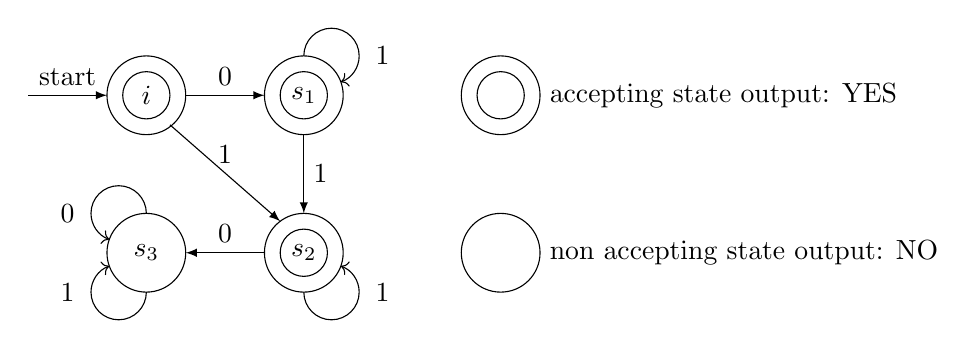
\begin{tikzpicture}
				% Top arrows
				\draw[-latex] (-2, 0)--node[above]{start} (-1, 0);
				\draw[-latex] (0, 0)--node[above]{0} (1, 0);
				% Bottom arrow
				\draw[latex-] (0, -2)--node[above]{0} (1, -2);
				% Middle arrows
				\draw[-latex] (-0.2, -0.375)--node[above]{1} (1.2, -1.6);
				\draw[-latex] (1.5, -0.5)--node[right]{1} (1.5, -1.5);
				
				% Circles
				% Top Left
				\draw (-0.5, 0) circle [radius=0.5];
				\draw (-0.5, 0) circle [radius=0.3] node{$i$};
				
				% Top right
				\draw (1.5, 0) circle [radius=0.5];
				\draw (1.5, 0) circle [radius=0.3] node{$s_1$};
				\draw[->] (1.5, 0.5)  arc(180:-70:10pt);
				\draw (2.5, 0.5) node{1};
				
				% Bottom left
				\draw (-0.5, -2) circle [radius=0.5] node{$s_3$};
				\draw[->](-0.5, -2.5) arc(0:-250:10pt);
				\draw[->](-0.5, -1.5) arc(0:250:10pt);
				\draw (-1.5, -2.5) node{1};
				\draw (-1.5, -1.5) node{0};
				
				% Bottom right
				\draw (1.5, -2) circle [radius=0.5];
				\draw (1.5, -2) circle [radius=0.3] node{$s_2$};
				\draw[->](1.5, -2.5) arc(-180:70:10pt);
				\draw (2.5, -2.5) node{1};
				
				% Legend
				\draw (4, 0) circle [radius=0.5];
				\draw (4, 0) circle [radius=0.3];
				\draw (4.5, 0) node[right]{accepting state output: YES};
				
				\draw (4, -2) circle [radius=0.5];
				\draw (4.5, -2) node[right]{non accepting state output: NO};
			\end{tikzpicture}
		\end{figure}
		~\\
		Accepting states in this examples: $i, s_1, s_2$ \\
		Non accepting states: $s_3$ \\
		Start states: $i$ \\
		Here $S = \{i, s_1, s_2, s_3\} \hspace{5mm} F = \{i, s_1, s_2\} \hspace{5mm} A = \{0, 1\} \hspace{5mm} t: S \times A \rightarrow S \hspace{5mm} t(i, 0) = s_1 \hspace{5mm} t(i, 1) = s_2 \hspace{5mm} t(s_1, 0)  = s_1 \hspace{5mm} t(s_1, 1) = s_2 \hspace{5mm} t(s_2, 0) = s_3 \hspace{5mm} t(s_2, 1) = s_2$ \\
		Let's process some strings:
		\begin{table}[h!]
			\centering
			\begin{tabular}{c|ccc|c|c|c|c|c}
				\cline{1-2} \cline{4-9}
				String & $\varepsilon$ (empty string) & & String & 0 & 0 & 1 & 1 & 1 \\ \cline{1-2} \cline{4-9}
				State (i) & i & & State i & $s_1$ & $s_1$ & $s_2$ & $s_2$ & $s_2$ \\ \cline{1-2} \cline{4-9}
				Output & YES & & Output & \multicolumn{5}{c}{YES} \\ \cline{1-2} \cline{4-9}
			\end{tabular}
		\end{table}
		\begin{table}[h!]
			\centering
			\begin{tabular}{c|c|ccc|ccc|c|c|c|c}
				\cline{1-3} \cline{5-6} \cline{8-12}
				String & 1 & 1 & & String & 1 & & String & 0 & 1 & 0 & 1 \\ \cline{1-3} \cline{5-6} \cline{8-12}
				State i & $s_2$ & $s_2$ & & State i & $s_2$ & & State i & $s_1$ & $s_2$ & $s_3$ & $s_3$ \\ \cline{1-3} \cline{5-6} \cline{8-12}
				Output & \multicolumn{2}{c}{YES} & & Output & YES & & Output & \multicolumn{4}{c}{NO} \\ \cline{1-3} \cline{5-6} \cline{8-12}
			\end{tabular}
		\end{table}
		~\\
		Now that we really understand what a finite state acceptor is, we can develop a criterion for recognised regular languages called the \underline{Myhill-Nerode theorem} based on an equivalence relation we can set up on words in our language over the alphabet $A$.
		\item[Definition:] Let $x, y \in L$, a language over the alphabet $A$. We call $x$ and $y$ equivalent over $L$ denoted by $x \equiv_L y$ if $\forall w \in A*, xw \in L \Leftrightarrow yx \in L$.
		\item[Note:] $xw$ means the concatenation $x \circ w$, and $yw$ is the concatenation $y \circ w$.
		\item[Idea:] If $x \equiv_L y$, then $x$ and $y$ place our finite state acceptor into the \underline{same state} $s$.
		\item[Notation:] Let $L/N$ be the set of equivalence classes determined by the equivalence relation $\equiv_L$.
		\item[The Myhill-Nerode Theorem:] Let $L$ be a language over the alphabet $A$. If the set $L/N$ ofequivalence classes in $L$ is infinite, then $L$ is not a regular language.
		\item[Stretch of Proof:] All element of one equivalence class in $L/N$ place our automation into the same state $s$. Elements of distinct equivalence classes place the automation into distinct state, \textbf{i.e.} if $[x], [y] \in L/N$ and $[x] \neq [y]$, then all elements of $[x]$ place the automation into some state $s$, while all elements of $[y]$ place the automation into some state $s'$, with $s \neq s' \Rightarrow$ an automation that can recognise $L$ has \underline{as many} states at the number of equivalence classes in $L/N$, but $L/N$ is \underline{NOT} finite $\Rightarrow L$ cannot be recognised by a finite state automation $\Rightarrow L$ is not regular by the theorem above.
		\item[qed]
	\end{description}
	
	\section{Regular Grammars}
	\begin{description}
		\item[Task:] Understand what is the form of the production rules of a grammar that generates a regular language.
		\item[Recall:] that a context-free grammar is given by $(V, A {<}s{>}, P)$ where every production rule $<$T$> \rightarrow w$ in $P$ causes \underline{one and only one} nonterminal to be replaced by a string in $V*$.
		\item[Definition:] A context-free grammar $(V, A {<}s{>}, P)$ is called a \underline{regular grammar} is every production rule in $P$ is of one of the three forms:
		\begin{enumerate}
			\item[(i)] $<$A$> \rightarrow$ b$<$B$>$
			\item[(ii)] $<$A$> \rightarrow$ b
			\item[(iii)] $<$A$> \rightarrow \varepsilon$
		\end{enumerate}
		where $<$A$>$ and $<$B$>$ are nonterminals, $b$ is a terminal, and $\varepsilon$ is the empty word. A regular grammar is said to be in normal form if all its production rules are of types (i) and (iii).
		\item[Remark:] In the literature, you often see this definition labelled \underline{left-regular grammar} as opposed to \underline{right-regular grammar}, where the production rules of types 1 have the form $<$A$> \rightarrow <$B$>$b, (\textbf{i.e.} the termminal is one the right of the nonterminal). This distinction is not really important as long as we stick to one type throughout since both \underline{left regular grammars} and \underline{right regular grammars} generate regular languages.
		\item[Lemma:] Any language generated by a regular grammar may be generated by a regular grammar in normal form.
		\item[Proof:] Let $<$A$> \rightarrow$b be a rule of type (ii). Replace it by two rules: $<$A$> \rightarrow$b$<$F$>$ and $<$F$> \rightarrow \varepsilon$, where $<$F$>$ s a new nonterminal. Add $<$F$>$ to the set $V$. We do the same for every rule of type (ii) obtaining a bigger set $V$, but now our production rules are only of type (i) and (iii) and we are generating the same language.
		\item[qed]
		\item[Example:] Recall the regular language $L = \{0^m1^n \mid m, n \in \mathbb{N}, m \geq 0, n \geq 0 \}$. We can generate it from the regular grammar in normal gorm given by production rules:
		\begin{enumerate}
			\item $<$s$> \rightarrow$ 0$<$A$>$
			\item $<$A$> \rightarrow$ 0$<$A$>$
			\item $<$A$> \rightarrow \varepsilon$
			\item $<$s$> \rightarrow \varepsilon$
			\item $<$A$> \rightarrow$ 1$<$B$>$
			\item $<$B$> \rightarrow$ 1$<$B$>$
			\item $<$s$> \rightarrow$ 1 $<$B$>$
			\item $<$B$> \rightarrow \varepsilon$
		\end{enumerate}
		Rules (1), (2), (5), (6), (7) are of type (i), where rules (3), (4) and (8) are of types (iii). \\
		(1) and (3) gives 0. (1), (2) applied $m-1$ times and (3) gives $0^m$ for $m \geq 2$. \\
		(7) and (8) give 1. (7), (6) applied $n-1$ times and (8) give $1^n$ for $n \geq 2$. \\
		(1), (5) and (8) give 01. (1), (5), (6) applied $n-1$ times and (8) gives $01^n$ for $n \geq 2$. \\
		(1), (2) applied $m-1$ times, (5) and (8) gives $0^m1$ for $m \geq 2$. \\
		(1), (2) applied $m-1$ times, (5), (6) applied $n-1$ times, and (8) gives $0^m1^n$ for $m \geq 2, n \geq 2$. \\
		Rule (4) gives the empty word $\varepsilon = 0^01^0$.
		\item[Q:] Why does a regular grammar yield a regular language, \textbf{i.e.} one recognised by a finite state acceptor?
		\item[A:] Not obvious from the definition, \underline{but} we can construct the finite state acceptor from the regular grammar as follows: our regular grammar is given by $(V, A, {<}s{>}, P)$.  \underline{Want} a finite state acceptor $(S, A, i, t, F)$. Immediately, we see the alphabet $A$ is the same and $i=<$s$>$. This gives us the idea of associating to every nonterminal symbol in $B \backslash A$ a state. $<$s$> \in V \backslash A$, so that's good. Next we ask:
		\item[Q:] Is it sufficient for $S = V \backslash A$?
		\item[A:] No! Our set $F$ of finishing/accepting states should be nonempty. So we add an element $\{f\}$ to $V \backslash A$, where our acceptor will end up when a word in our language. Thus, $S = (V \backslash A) \cup \{f\}$ and $F \{f\}$. $F \subseteq S$ as needed.
		\item[Q:] How do we define $t$?
		\item[A:] Use the production rules in $P$! For every rule of type (i), which is of the form $<$A$> \rightarrow$ b$<$B$>$ set $t(<$A$>$,b$) = <$B$>$. This works out well because our nonterminals $<$A$>$ and $<$B$>$ are states of the acceptor and the terminal $b \in A$ for $t$ takes an element of $S \times A$ to an element of $S$ as needed. Now look at production rules of type (ii), $<$A$> \rightarrow b$ and of types (iii), $<$A$> \rightarrow \varepsilon$. Those are applied when we \underline{finish} constructing a word $w$ in our language $L$, \textbf{i.e.} at the very last step, so our acceptor should end up in the finishing state $f$ whenever a production rule of type (ii) or (iii) is applied. Write a production rule of type (ii) or (iii) as $<$A$> \rightarrow w$, then we can set $t(<$A$>, w) = f$. We have finished constructing $t$ as well. Technically, $t:S \times (A \cup \{ \varepsilon \}) \rightarrow S$ instead of $t:S \times A \rightarrow S$, but we can easily fix the transition function t by combining the last two transitions for each accepted word.
		\item[Remark:] The same general principals as we used above allow us to go from a finite state acceptor to a regular grammar. This gives us the following theorem:
		\item[Theorem:] A language $L$ is regular $\Leftrightarrow L$ is recognised by a finite state acceptor $\Leftrightarrow L$ is generated by a regular grammar.
	\end{description}
	
	\subsection{Applications of Formal Languages and Grammars as well as Automata Theory}
	\begin{enumerate}
		\item Compiler architecture uses context-free grammars
		\item Parsers - recognise if commands comply with the syntax of a language
		\item Pattern matching and data mining - guess the language from a given set of words (applied in CS, etc)
		\item Natural language processing - example in David Wilkins' notes pp40-44
		\item Checking proofs by computers/automatic theorem proving - simpler example of this kind in David Wilkins' notes pp45-57 that pertains to propositional logic
		\item Theory of regular expressions (related to the definition of a regular language that we gave) enables
		\begin{enumerate}
			\item grep/awk/sed in Unix
			\item More efficient coding (avoiding unnecessary detoirs in your code)
		\end{enumerate}
		\item Biology - John Conway's game of life is a cellular automation
		\item Modelling of AI characters in games uses the finite state automation idea. Our character can choose among different behaviours based on stimuli - like a finite state automation reacting to input
		\item Strategy and tactics in games - teach the opposition to recognise certain patterns, then suddenly change them to gain an advantage and score - used in football, fencing, etc.
		\item Learning a sport/a numerical instrument/a new field or subject - split the information into blocks and learn how to combine them into meaningful patterns - uses notions from context-sensitive grammars.
		\item Finite state automata and probability - chaos theory, financial mathematics.
		\item[etc...]
	\end{enumerate}
	
	\section{Graph Theory}
	\begin{description}
		\item[Task:] Introduce terminology related to graphs; understand different types of graphs; learn how to put together arguments involving graphs. \\
		An \underline{undirected graph} consists of:
		\begin{enumerate}
			\item A finite set of points $V$ called \underline{vertices}
			\item A finite set $E$ of \underline{edges} joining two distinct vertices of the graph.
		\end{enumerate}
		\item[Understand the meaning of an edge better:] Let $V$ be the set of vertices. Consider $P(V)$, the power set of $V$. Let $V_2 \subseteq P(V)$ consist of all subsets of $V$ containing exactly 2 points, \textbf{i.e.} $V_2 = \{A \in P(V) \mid \#(A)=2 \}$ \\
		Identify each element in $V_2$ with the edge joining the two points. In other words, if $\{a, b\} \in V_2$, then we can let $ab$ be the edge corresponding to $\{1, b\}$.
		\item[Examples:]
		\begin{enumerate}
			\item[]
			\item A traingle is an undirected graph. \\
			\begin{figure}[h!]
				\centering
				\begin{tikzpicture}
					\draw (0, 0) node[above]{A} -- (-1, -2);
					\draw (0, 0) -- (3, -2) node[right]{C};
					\draw  (-1, -2) node[left]{B} -- (3, -2);
				\end{tikzpicture}
			\end{figure}
			$V = \{A, B, C\}$ \\
			3 possible 2 element subsets of $V$:
			$\{A, B\} \rightarrow AB$ \\
			$\{A, C\} \rightarrow AC$ \\
			$\{B, C\} \rightarrow BC$ \\
			$E = \{AB, AC, BC\}$
			\item A pentagram is an example of an undirected graph. \\
			\begin{figure}[h!]
				\centering
				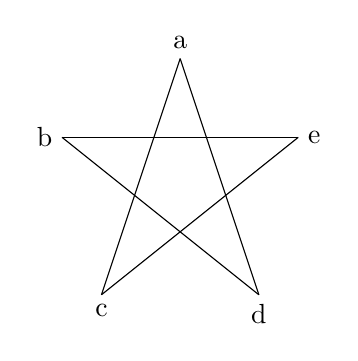
\begin{tikzpicture}
					\coordinate (A) at (0, 0);
					\coordinate (B) at (-1.5, -1);
					\coordinate (E) at (1.5, -1);
					\coordinate (C) at (-1, -3);
					\coordinate (D) at (1, -3);
					
					\draw (A) node[above]{a}--(C) node[below]{c};
					\draw (A)--(D) node[below]{d};
					\draw (C)--(E);
					\draw (D)--(B) node[left]{b};
					\draw (B)--(E) node[right]{e};
				\end{tikzpicture}
			\end{figure}
			$V = {a, b, c, d, e}$ \\
			$E = \{ac, ad, be, ce, bd\}$
		\end{enumerate}
		\item[Convention:] The set of vertices cannot be empty, \textbf{i.e.} $V \neq 0$.
		\item[Q:] If $V \neq \emptyset$, what is the simplest possible undirected graph?
		\item[A:] A graph consisting of a single point, \textbf{i.e.} with one vertex and two edges.
		\item[Definition:] A graph is called \underline{trivial} if it consists of one vertex and zero edges. Next, study how vertices and edges relate to each other.
		\item[Definition:] If $v$ is a vertex of some graph, if $e$ is an edge of that graph, and it $e = vv'$ for $v'$ another vertex, then the vertex $v$ is called \underline{incident} to the edge $e$ and the edge $e$ is called incident to the vertex $v$.
		\item[Example:] ~\\
		$b$ is incident to edges $be$ and $bd$ \\
		$be$ is incident to vertices $b$ and $e$
		\begin{figure}[h!]
			\centering
			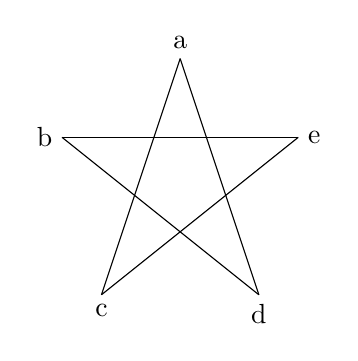
\begin{tikzpicture}
			\coordinate (A) at (0, 0);
			\coordinate (B) at (-1.5, -1);
			\coordinate (E) at (1.5, -1);
			\coordinate (C) at (-1, -3);
			\coordinate (D) at (1, -3);
			
			\draw (A) node[above]{a}--(C) node[below]{c};
			\draw (A)--(D) node[below]{d};
			\draw (C)--(E);
			\draw (D)--(B) node[left]{b};
			\draw (B)--(E) node[right]{e};
			\end{tikzpicture}
		\end{figure}
		\item[Definition:] Let $(V,E)$ be an undirected graph. Two vertices $A, B \in V \hspace{5mm} A \neq B$ are called \underline{adjacent} if $\exists$ edge $AB \in E$. \\
		We represent the incidence relations among the vertices $V$ and edges $E$ of an undirected graph via:
		\begin{enumerate}
			\item An incidence table
			\item An incidence matrix
		\end{enumerate}
		\item[Legend:] ~\\
		1 an incidence relation holds \\
		0 an incidene relation does not hold \\
		\item From the pentagram: \\
		$V = \{a, b, c, d, e\}$ \\
		$E = \{ac, ad, be, bd, ce\}$ \\
		\pagebreak
		\begin{figure}[h!]
			\centering
			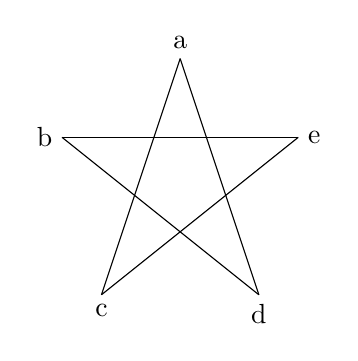
\begin{tikzpicture}
			\coordinate (A) at (0, 0);
			\coordinate (B) at (-1.5, -1);
			\coordinate (E) at (1.5, -1);
			\coordinate (C) at (-1, -3);
			\coordinate (D) at (1, -3);
			
			\draw (A) node[above]{a}--(C) node[below]{c};
			\draw (A)--(D) node[below]{d};
			\draw (C)--(E);
			\draw (D)--(B) node[left]{b};
			\draw (B)--(E) node[right]{e};
			\end{tikzpicture}
		\end{figure}
		\item The indidence table is:
		\begin{table}[h!]
			\centering
			\begin{tabular}{c|ccccc}
				& ac & ad & be & bd & ce \\ \cline{1-6}
				a & 1 & 1 & 0 & 0 & 0 \\
				b & 0 & 0 & 1 & 1 & 0 \\
				c & 1 & 0 & 0 & 0 & 1 \\
				d & 0 & 1 & 0 & 1 & 0 \\
				e & 0 & 0 & 1 & 0 & 1 \\
			\end{tabular}
		\end{table}
		\item Correspondingly, the incidence matrix is:
		\[ \left( \begin{array}{ccccc}
		1 & 1 & 0 & 0 & 0 \\
		0 & 0 & 1 & 1 & 0 \\
		1 & 0 & 0 & 0 & 1 \\
		0 & 1 & 0 & 1 & 0 \\
		0 & 0 & 1 & 0 & 1 \end{array} \right)\] 
		Note that for the incidence matrix to make sense, we need to know that vertices were considered in the order $\{a, b, c, d, e\}$ and edges in the order $\{ac, ad, be, bd, ce\}$. If we shuffle either set, the incidence matrix chances. \\
		With this in mind, we can now rigorously define the incidence matrix:
		\item[Definition:] Let $(V, E)$ be an undirected graph with $m$ vertices and $n$ edges. Let vertices be ordered as $v_1, v_2,..., v_m$, and let the edges be ordered $e_1, e_2, ..., e_n$. The \underline{incidence matrix} for such a graph is given by $\left( \begin{array}{cccc}
			a_{11} & a_{12} & ... & a_{1n} \\
			a_{21} & a_{22} & ... & a_{2n} \\
			\vdots & \vdots & \ddots & \vdots \\
			a_{m1} & a_{m2} & ... & a_{mn} \end{array} \right)$, where the entry $a_{ij}$ in row $i$ and column $j$ has the value 1 if the $i^{th}$ vertex is incident to the $j^{th}$ edge and has value 0 otherwise. \\
			Similarly, we can define the \underline{adjacency table} and the \underline{adjacency matrix} of a graph:
			\item[Definition:] Let $(V,E)$ be an undirected graph with $m$ vertices, and let these vertices be ordered as $v_1, v_2, ..., v_m$. The \underline{adjacency matrix} for this graph is given by $\left( \begin{array}{cccc}
			b_{11} & b_{12} & ... & b_{1m} \\
			b_{21} & b_{22} & ... & b_{2m} \\
			\vdots & \vdots & \ddots & \vdots \\
			b_{m1} & b_{m2} & ... & b_{mm} \end{array} \right)$ where $b_{ij}=1$ if $v_i$ and $v_j$ are adjacent to each other and $b_{ij}=0$ if $v_i$ and $v_j$ are not adjacent to each other.
			\item[Remark:] "Being adjacent to" is a symmetric relation on he set of vertices $V$, so the adjacency matrix is symmetric, \textbf{i.e.} $b_{ij}=b_{ji} \hspace{5mm} \forall i, j \hspace{5mm} 1 \leq i, j \leq m$. It is not reflexive so all the entries on the diagonal are zero.
	\end{description}
	
	\subsection{Complete graphs}
	\begin{description}
		\item[Definition:] A graph $(V, E)$ is called \underline{complete} if $\forall v, v' \in V$ s.t. $v \neq v'$, the edge $vv' \in E$. In other words, a complete grapg has the highest number of edges possible given its number of vertices.
		\item[Examples:] ~\\
		\begin{enumerate}
			\item The triangle is a complete graph.
			\item The pentagram is \underline{not} a complete graph.
		\end{enumerate}
		\item[Notation:] A complete graph with $n$ vertices is denoted by $K_n$.
		\item[Q:] How does the adjacency matrix of a complete graph look like?
		\item[A:] All entrices are 1 except on the diagonal, where they are all two.
		\item[Definition:] A graph $(V, E)$ is called \underline{bipartite} is $\exists$ subsets $V_1$ and $V_2$ s.t.
		\begin{enumerate}
			\item $V_1 \cup V_2 = V$
			\item $V_1 \cap V_2 = \emptyset$
			\item Every edge in $E$ is of the form $vw$ with $v \in V_1$ and $w \in V_2$.
		\end{enumerate}
		A bipartite graph is called a \underline{complete bipartite graph} if $\forall v \in V_1 \hspace{5mm} \forall w \in V_2 \hspace{5mm} \exists vw \in E$.
		\item[Notation:] A complete bipartite graph where the set $V_1$ has $p$ elements and the set $V_2$ has $q$ elements is denoted by $K_{p,q}$.
		\item[Example:] ~\\
		$V_1 = \{a, b\}$ \\
		$V_2 = \{c, d, e\}$ \\
		$V = \{a, b, c, d, e\}$ \\
		$E = \{ac, ad, ae, bc, bd, be\}$ \\
		\pagebreak
		\begin{figure}[h!]
			\centering
			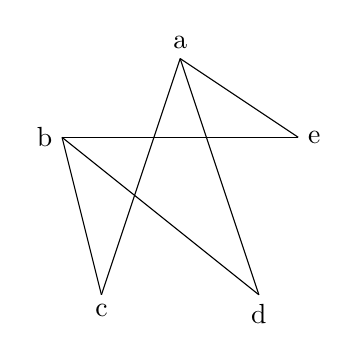
\begin{tikzpicture}
			\coordinate (A) at (0, 0);
			\coordinate (B) at (-1.5, -1);
			\coordinate (E) at (1.5, -1);
			\coordinate (C) at (-1, -3);
			\coordinate (D) at (1, -3);
			
			\draw (A) node[above]{a}--(C) node[below]{c};
			\draw (A)--(D) node[below]{d};
			\draw (A)--(E);
			\draw (B)--(C);
			\draw (D)--(B) node[left]{b};
			\draw (B)--(E) node[right]{e};
			\end{tikzpicture}
		\end{figure}
		is a complete bipartite graph.
		\item Next, relate graph to each other via functions with special properties.
	\end{description}
	
	\section{Isomorphism of Graphs}
	\begin{description}
		\item[Definition:] An \underline{isomorphism} between two graphs $(V, E)$ and $(V',E')$ is a bijective function $\varphi : V \rightarrow V'$ satisfying that $\forall a, b \in V$ with $a \neq b$ the edge $ab \in E \Leftrightarrow$ the edge $\varphi (a) \varphi (b) \in E'$.
		\item[Recall:] A function $\varphi : V \rightarrow V'$ is bijective $\Leftrightarrow$ it has an inverse $\varphi^{-1} : V' \rightarrow V'$. \\
		The bijection $\varphi V \rightarrow V'$ that gives the isomorphism between $(V, E)$ and $(V' E')$ thus sets up the following:
		\begin{enumerate}
			\item A 1-1 correspondence of the vertices $V$ of $(V,E)$ with the vertices $V'$ of $(V',E') \rightarrow$ comes from $\varphi: V \rightarrow V'$ being bijective.
			\item A 1-1 correspondence of the edges $E$ of $(V,E)$ with the edges $E'$ of $(V',E') \rightarrow$ comes from the additional property in the definition of an isomorphism that $\forall a, b \in V$ with $a \neq b, ab \in E \Leftrightarrow \varphi (a) \varphi (b) \in E'$. 
		\end{enumerate}
		\item[Remark:] Just like an isomorphism of groups discussed earlier in the course, an ismorphism of graphs means $(V,E)$ and $(V',E')$ have the same "iso" from "morph\'{e}". "Being isomorphic" is an equivalence relations, so we get classes of graphs that have the same form as our equivalence classes.
		\item[Definition:] If there exists an isomorphism $\varphi :V \rightarrow V'$ between two graphs $(V, E)$ and $(V', E')$, then $(V, E)$ and $(V', E')$ are called isomorphic.
	\end{description}
	
	\section{Subgraphs}
	\begin{description}
		\item[Task:] Understand subobjects of a graph.
		\item[Definition:] Let $(V, E)$ and $(V', E')$ be graphs. The graph $(V', E')$ is called a subgraph of $(V, E)$ if $V' \subseteq V$ and $E' \subseteq E$, \textbf{i.e.} if $(V', E')$ consists of a subset $V'$ of the vertices of $(V, E)$ and a subset $E'$ of edges $(V, E)$ between vertices in $V'$.
		\item[Example:] Star of David on the flag of Israel \\
			$V = \{a, b, c, d, e, f\}$ \\
			$E = \{ac, ce, ae, bf, fd, bd\}$ \\
			\begin{figure}[h!]
				\centering
				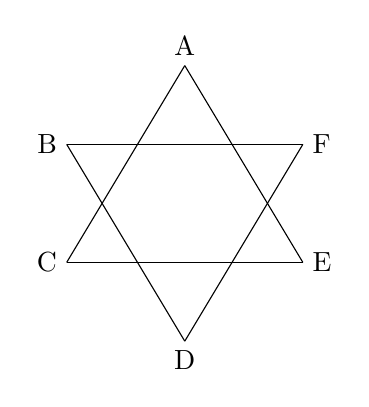
\begin{tikzpicture}
				\coordinate (A) at (0, 0);
				\coordinate (B) at (-1.5, -1);
				\coordinate (C) at (-1.5, -2.5);
				\coordinate (D) at (0, -3.5);
				\coordinate (E) at (1.5, -2.5);
				\coordinate (F) at (1.5, -1);
				
				\draw (A) node[above]{A} -- (C);
				\draw (A) -- (E) node[right]{E};
				\draw (C) node[left]{C} -- (E);
				\draw (D) -- (B) node[left]{B};
				\draw (D) node[below]{D} -- (F);
				\draw (B) -- (F) node[right]{F};
			\end{tikzpicture}
		\end{figure}
		\item 2 triangle subgraphs of the star of David: \\
		\begin{tabular}{ll}
				$V' = \{a, c, e\}$ & $E' = \{ac, ce, ae\}$ \\
				$V" = \{b, f, d\}$ & $E" = \{bf, fd, bd\}$
		\end{tabular}
	\end{description}
	
	\section{Vertex Degrees}
	\begin{description}
		\item[Task:] Use numbers to understand incidence relationships.
		\item[Definition:] Let $(V, E)$ be a graph. The \underline{degree} deg $v$ of a vertex $v \in V$ is defined as the number of edges of the graph that are incidence to $v$, \textbf{i.e.} the number of edge with $v$ as one of their endpoints.
		\item[Example:] ~\\
		\begin{figure}[h!]
			\centering
			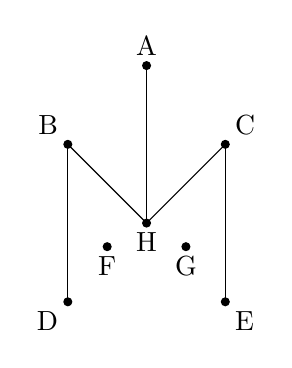
\begin{tikzpicture}
			\coordinate (A) at (0, 0);
			\coordinate (H) at (0, -2);
			\coordinate (B) at (-1, -1);
			\coordinate (C) at (1, -1);
			\coordinate (D) at (-1, -3);
			\coordinate (E) at (1, -3);
			\coordinate (F) at (-0.5, -2.3);
			\coordinate (G) at (0.5, -2.3);
			
			\draw (A) -- (H);
			\draw (H) -- (B);
			\draw (H) -- (C);
			\draw (B) -- (D);
			\draw (C) -- (E);
			
			\draw[fill=black] (A) circle[radius=0.5mm] node[above]{A};
			\draw[fill=black] (B) circle[radius=0.5mm] node[above left]{B};
			\draw[fill=black] (C) circle[radius=0.5mm] node[above right]{C};
			\draw[fill=black] (D) circle[radius=0.5mm] node[below left]{D};
			\draw[fill=black] (E) circle[radius=0.5mm] node[below right]{E};
			\draw[fill=black] (H) circle[radius=0.5mm] node[below]{H};
			\draw[fill=black] (F) circle[radius=0.5mm] node[below]{F};
			\draw[fill=black] (G) circle[radius=0.5mm] node[below]{G};
			\end{tikzpicture}
		\end{figure}
		~\\
		def $f$ = deg $g$ = 0 \\
		deg $d$ = deg $e$ = deg $a$ = 1 \\
		deg $b$ = deg $c$ = 2 \\
		deg $h$ = 3 \\
		\item[Definition:] A vertex of degree 0 is called an \underline{isolated} vertex.
		\item[Definition:] A vertex of degree 1 is called a \underline{pendent} vertex.
		\item[Theorem:] Let $(V, E)$ be a graph. Then $\sum_{v \in V}$deg $v = Z\#(E)$, where $\sum_{v \in V}$deg $v$ is the sum of the degrees of all the vertices of the graph, and $\#(E)$ is the number of edges of the graph.
		\item[Proof:] $\sum_{v \in V}$deg $v$ is the sum of all the entries in the adjacency matrix. Every edge $vv' \in E$ contributes 2 to the sum $\sum_{v \in V}$deg $v$, 1 for the vertex $v$ and 1 for the vertex $v' \Rightarrow$ each edge must be counted twice, so $\sum_{v \in V}$deg $v = 2 \#(E)$.
		\item[qed]
		\item[Corollary:] $\sum_{v \in V}$deg $v$ is an even integer.
		\item[Proof:] Since $\sum_{v \in V}$deg $v = 2 \#(E)$, and $\#(E) \in \mathbb{N}$, the result follows.
		\item[qed]
		\item[Corollary:] In any graph, the number of vertices of odd degrees must be even.
		\item[Proof:] Assume not, then $\sum_{v \in V}$deg $v$ is an odd integer as $odd + even = odd \Rightarrow \Leftarrow$ to the previous corollary.
		\item[qed]
		\item[Definition:] A graph is called k-regular for some non-negative integer $k$ if every vertex of the graph has degree equal to $k$.
		\item[Example:] A rectangle is 2-regular. \\
		\begin{figure}[h!]
			\centering
			\begin{tikzpicture}
				\coordinate (A) at (0, 0);
				\coordinate (B) at (4, 0);
				\coordinate (D) at (0, -2);
				\coordinate (C) at (4, -2);
				
				\draw (A) node[above left]{A} -- (B);
				\draw (A) -- (D) node[below left]{D};
				\draw (B) node[above right]{B} -- (C);
				\draw (D) -- (C) node[below right]{C};
			\end{tikzpicture}
		\end{figure}
		deg $a$ = deg $b$ = deg $c$ = deg $d$ = 2.
		\item[Definition:] A graph $(V, E)$ is called \underline{regular} is $\exists k \in \mathbb{N}$ s.t. $(V, E)$ is k-regular.
		\item[Corollary:] Let $(V, E)$ be a k-regular graph. Then $k\#(V) = 2\#(E)$ where $\#(V)$ is the number of vertices and $\#(E)$ is the number of edges.
		\item[Proof:] By the theorem, $\sum_{v \in V}$deg $v = 2\#(E)$, but $(V, E)$ is k-regular $\Rightarrow$ deg $v = k \forall v \in V$. Therefore $\sum_{v \in V}$deg $v = \#(V).k = 2 \#(E)$.
		\item[qed]
		\item[Example:] Consider a complete graph $(V, E)$ with $n$ vertices. $(V, E)$ is $(n-1)$-regular because every vertex is adjacent to all the remaining $(n-1)$ vertices.
		\item[Corollary:] A complete bipartite graph $k_{p,q}$ is regular $\Leftrightarrow p = q$
		\item[Proof:] Recall that $V=V_1 \cup V_2 \hspace{10mm} V_1 \cap V_2 = \emptyset$ for a bipartite graph. \\
		$\Leftarrow$ is $p=q, \forall v \in V_1$ satisfies that deg $v = p = q$ and $\forall v \in V_2$ satisfies that def $v=p=q$ since the graph is complete $\Rightarrow (V, E)$ is p-regular. \\
		$\Rightarrow \: (V, E)$ is regular $\Rightarrow \forall v \in V_1$ and $\forall v' \in V_2$, deg $v=$ deg $v'$, but $(V, E)$ is complete $\Rightarrow v$ is adjacent to all vertices in $V_2$, \textbf{i.e.} def $v = \#(V_1)$ and $v'$ is adjacent to all vertices in $V_1$, \textbf{i.e.} deg $v' = \#(V_2) \rightarrow \#(V_1) = \#(V_2)$
	\end{description}
	
	\section{Walks, trails and paths}
	\begin{description}
		\item[Task:] Make rigorous the notion of traversing parts of a graph in order to understand its structure better.
		\item[Definition:] Let $(V, E)$ be a graph. A \underline{walk} $v_0 v_1 v_2... v_n$ of length $n$ in the graph from vertex $a$ to vertex $b$ is determined by a finite sequence $v_0, v_1, v_1, ..., v_n$ of vertices of the graph s.t. $v_0 = a, v_n = b$ and $v_{i-1} v_i$ is an edge of the graph for $i=1, 2, ..., n$.
		\item[Definition:] A walk $v_0 v_1 v_2 ... v_n$ in a graph is said to \underline{traverse} the edges $v_{i-1} v_i$ and to \underline{pass through} the vertices $v_0, v_1, ..., v_n$. Length of walk $= \#$ of edges traversed $\rightarrow$ the smallest possible number is two edges. As a result, we have the following definition:
		\item[Definition:] A walk that consists of a single vertex $v \in V$ and has length two is called \underline{trivial}.
		\item[Definition:] Let $(V, E)$ be a graph. A \underline{trail} $v_0 v_1 v_2 ... v_n$ of length $n$ in the graph from some vertex $a$ to some vertex $b$ is a walk of length $n$ from $a$ to $b$ with the property that edges $v_{i-1} v_i$ are distinct for $i-1, 2, ..., n$. In other words, a trail is a walk in the graph, which traverses edges of the graph at most once.
		\item[Definition:] A walk, trail or path is a graph is called \underline{trivial} if it is a walk of length two consist of a single vertex $v \in V$; otherwise, the walk, trail, or path is called \underline{non-trivial}.
		\item[Example:] ~\\
		\begin{enumerate}
			\item $h$ is a trivial walk/trail/path
			\item $defd$ is a trail, but not a path because we pass through the vertex $d$ twice.
			\item $def$ is a path
			\item $gfdefdc$ is a walk but not a trail of a path
		\end{enumerate}
		\begin{figure}[h!]
			\centering
			\begin{tikzpicture}
			\coordinate (G) at (0, -1);
			\coordinate (F) at (3, -3.5);
			\coordinate (E) at (1, -3);
			\coordinate (D) at (1, -5);
			\coordinate (A) at (-2, -3.5);
			\coordinate (H) at (-1, -3.2);
			\coordinate (B) at (-0.5, -6.2);
			\coordinate (C) at (2.7, -7);
			
			\draw (G) -- (F) -- (D) -- (C) -- (B) -- (A) -- (G);
			\draw (D) -- (E) -- (F);
			
			\draw[fill=black] (A) circle[radius=0.5mm] node[left]{A};
			\draw[fill=black] (B) circle[radius=0.5mm] node[below left]{B};
			\draw[fill=black] (C) circle[radius=0.5mm] node[right]{C};
			\draw[fill=black] (D) circle[radius=0.5mm] node[left]{D};
			\draw[fill=black] (E) circle[radius=0.5mm] node[above]{E};
			\draw[fill=black] (F) circle[radius=0.5mm] node[right]{F};
			\draw[fill=black] (G) circle[radius=0.5mm] node[above]{G};
			\draw[fill=black] (H) circle[radius=0.5mm] node[above]{H};
			\end{tikzpicture}
		\end{figure}
	\end{description}
	
	\section{Connected Graphs}
	\begin{description}
		\item[Task:] Use the ideas above related to traversing parts of a graph in order to define a particularly important category of graphs.
		\item[Definition:] An undirected graph $(V, E)$ is called \underline{connected} if $\forall u, v \in V$ vertices, $\exists$ path in the graph from $u$ to $v$.
		\item[Examples:]
		\begin{enumerate}
			\item Is not connected as $d$ is not connected to any other vertex.
			\begin{figure}[h!]
				\centering
				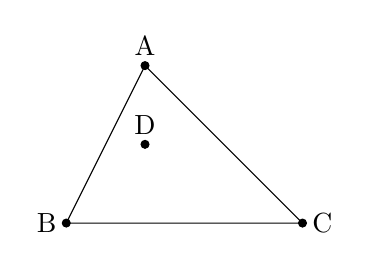
\begin{tikzpicture}
				\coordinate (A) at (0, 0);
				\coordinate (B) at (-1, -2);
				\coordinate (C) at (2, -2);
				\coordinate (D) at (0, -1);
				
				\draw (A) -- (B) -- (C) -- (A);
				\draw[fill=black] (A) circle[radius=0.5mm] node[above]{A};
				\draw[fill=black] (B) circle[radius=0.5mm] node[left]{B};
				\draw[fill=black] (C) circle[radius=0.5mm] node[right]{C};
				\draw[fill=black] (D) circle[radius=0.5mm] node[above]{D};
				\end{tikzpicture}
			\end{figure}
			\pagebreak
			\item Is connected. $\exists$ path between any two of the vertices.
			\begin{figure}[h!]
				\centering
				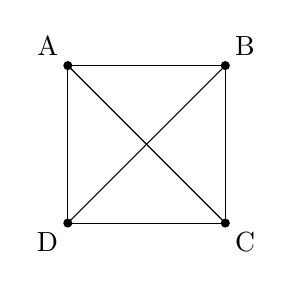
\begin{tikzpicture}
				\coordinate (A) at (-1, 1);
				\coordinate (B) at (1, 1);
				\coordinate (C) at (1, -1);
				\coordinate (D) at (-1, -1);
				
				\draw (A) -- (B) -- (C) -- (D) -- (A);
				\draw (A) -- (C);
				\draw (D) -- (B);
				
				\draw[fill=black] (A) circle[radius=0.5mm] node[above left]{A};
				\draw[fill=black] (B) circle[radius=0.5mm] node[above right]{B};
				\draw[fill=black] (C) circle[radius=0.5mm] node[below right]{C};
				\draw[fill=black] (D) circle[radius=0.5mm] node[below left]{D};
				\end{tikzpicture}
			\end{figure}
		\end{enumerate}
		\item[Theorem:] Let $(V, E)$ be a undirected graph, and let $u, v \in V. \exists$ path between $u$ and $v$ in the graph $\Leftrightarrow \exists$ walk in the graph between $u$ and $v$.
		\item[Proof:] $\Rightarrow$ trivial: A path is a walk. \\
		$\Leftarrow \exists$ walk between $u$ and $v$. Choose the walk of least length between $u$ and $v$, (\textbf{i.e.} $\nexists$ a walk of lower length than this one) and prove it is a path. Let this walk be $a_0 a_1 ... a_n$ with $a_0 = u$ and $a_n = v$. Assume $\exists j, k$ with $a \leq j, k \leq n$ s.t. $j < k$ and $a_j = a_k$, but then $a_0 a_1 ... a_j a_k+1 ... a_n$ would be a walk from $u$ to $v$ of \underline{strictly smaller} length than $a_0 a_1 ... a_n$. $\Rightarrow \Leftarrow$ as we chose $a_0 a_1 ... a_n$ to be of minimal length $ \Rightarrow a_i \neq a_j \forall i, j$ s.t. $0 \leq i, j \leq n \Rightarrow a_0 a_1 ... a_n$ is a path between $u$ and $v$.
		\item[qed]
		\item[Corollary:] An undirected grapg $(V, E)$ is connected $\Leftrightarrow \forall u, v \in V \exists$ walk in the graph between $u$ and $v$.
	\end{description}
	
	\section{Components of a graph}
	\begin{description}
		\item[Task:] Divide a graph into subgraphs that are isolated from each other.
	\end{description}
	Let $(V, E)$ be an undirected graph. We define a relation $\sim$ on the set of vertices $V$, where $a, b \in V$ satisfy $a \sim b$ iff $\exists$ walk in the graph from $a$ to $b$.
	\begin{description}
		\item[Lemma:] Let $(V, E)$ be an undirected graph. The relation $a \sim b$ or $a, b \in V$, which holds iff $\exists$ walk in the graph between $a$ and $b$ is an equivalence relation.
		\item[Proof:] We must show $\sim$ is reflexive, symmetric, and transitive.
		\item[Reflexive:] $\forall v \in V, v \sim v$ since the trivial walk is a walk from $v$ to itself.
		\item[Symmetric:] If $a \sim b$ for $a, b \in V$, then $\exists$ walk $v_0 v_1 ... v_n$ where $v_0 = a$ and $v_n = b$. This walk can be reversed to $v_n v_{n-1} ... v_1 v_0$, which now goes from $v_n = b$ to $v_0 = a$. Therefore, $b \sim b$ as needed.
		\item[Transitive:] If $a \sim b$ and $b \sim c$, for $a, b, c \in V$, there $\exists$ walk $a v_1 v_2 ... v_{n-1} b$ from $a$ to $b$ and $\exists$ walk $b w_1 w_2 ... w_{m-1} c$ from $b$ to $c$. We put these two walks together (concatenate them) to yield the walk $a v_1 v_2 ... v_{n-1} b w_1 w_2 ... w_{m-1} c$ from $a$ to $c$. Therefore $a \sim c$.
		\item[qed]
	\end{description}
\end{document}